% *****************************************************************************
% Dissertation template and document class for Princeton University
% Template Author  : Jeffrey Scott Dwoskin <jdwoskin@princeton.edu>
% Adapted from: http://www.math.princeton.edu/graduate/tex/puthesis.html
% ****************************************************************************%

% Author: Ben Eisner


% Single-spaced print copy
% \documentclass[12pt,lot, lof, singlespace]{sty/puthesis}
% \newcommand{\printmode}{}

% Double-spaced electronic copy
\documentclass[12pt,lot, lof]{sty/puthesis}
\newcommand{\proquestmode}{}

%% Draft w/o frontmatter
% \documentclass[12pt]{puthesis}

%%%%%%%%%%%%%%%%%%%%%%%%%%%%%%%%%%%%%%%%%%%%%%%%%%%%%%%%%%%%%
% Author & title page info

\title{Deep Learning methods for 3D segmentation of neural tissue in EM images}

\submitted{May 5, 2017}
\copyrightyear{2017} 
\author{Benjamin Eisner}
\adviser{Sebastian Seung} 
\department{Computer Science}

%%%%%%%%%%%%%%%%%%%%%%%%%%%%%%%%%%%%%%%%%%%%%%%%%%%%%%%%%%%%%\
%%%% Tweak float placements
% From: http://mintaka.sdsu.edu/GF/bibliog/latex/floats.html "Controlling LaTeX Floats"
% and based on: http://www.tex.ac.uk/cgi-bin/texfaq2html?label=floats
% LaTeX defaults listed at: http://people.cs.uu.nl/piet/floats/node1.html

% Alter some LaTeX defaults for better treatment of figures:
    % See p.105 of "TeX Unbound" for suggested values.
    % See pp. 199-200 of Lamport's "LaTeX" book for details.
    %   General parameters, for ALL pages:
    \renewcommand{\topfraction}{0.85}	% max fraction of floats at top
    \renewcommand{\bottomfraction}{0.6}	% max fraction of floats at bottom
    %   Parameters for TEXT pages (not float pages):
    \setcounter{topnumber}{2}
    \setcounter{bottomnumber}{2}
    \setcounter{totalnumber}{4}     % 2 may work better
    \setcounter{dbltopnumber}{2}    % for 2-column pages
    \renewcommand{\dbltopfraction}{0.66}	% fit big float above 2-col. text
    \renewcommand{\textfraction}{0.15}	% allow minimal text w. figs
    %   Parameters for FLOAT pages (not text pages):
    \renewcommand{\floatpagefraction}{0.66}	% require fuller float pages
	% N.B.: floatpagefraction MUST be less than topfraction !!
    \renewcommand{\dblfloatpagefraction}{0.66}	% require fuller float pages

% The documentclass already sets parameters to make a high penalty for widows and orphans. 

%%%%%%%%%%%%%%%%%%%%%%%%%%%%%%%%%%%%%%%%%%%%%%%%%%%%%%%%%%%%%\
%%%% Use packages

%\usepackage{amsfonts}

%%% For figures
\usepackage{graphicx}
\usepackage{amsmath,bm}
%\usepackage{subfig,rotate}

%%% for comments
\usepackage{verbatim}

%%% For tables
\usepackage{multirow}
% Longtable lets you have tables that span multiple pages.
\usepackage{longtable}

% Booktabs produces far nicer tables than the standard LaTeX tables.
%   see: http://en.wikibooks.org/wiki/LaTeX/Tables
\usepackage{booktabs}

\usepackage{color}

\usepackage{geometry}

\usepackage{listings}

\usepackage{caption}
\usepackage{subcaption}
\usepackage{tabularx}

\definecolor{codegreen}{rgb}{0,0.6,0}
\definecolor{codegray}{rgb}{0.5,0.5,0.5}
\definecolor{codepurple}{rgb}{0.58,0,0.82}
\definecolor{backcolour}{rgb}{0.95,0.95,0.92}
 
\lstdefinestyle{mystyle}{
    backgroundcolor=\color{backcolour},   
    commentstyle=\color{codegreen},
    keywordstyle=\color{magenta},
    numberstyle=\tiny\color{codegray},
    stringstyle=\color{codepurple},
    basicstyle=\footnotesize,
    breakatwhitespace=false,         
    breaklines=true,                 
    captionpos=b,                    
    keepspaces=true,                 
    numbers=left,                    
    numbersep=5pt,                  
    showspaces=false,                
    showstringspaces=false,
    showtabs=false,                  
    tabsize=2
}
 
\lstset{style=mystyle}

%set parameters for longtable:
% default caption width is 4in for longtable, but wider for normal tables
\setlength{\LTcapwidth}{\textwidth}



%%%%%%%%%%%%%%%%%%%%%%%%%%%%%%%%%%%%%%%%%%%%%%%%%%%%%%%%%%
%%% Printed vs. online formatting
\ifdefined\printmode

% Printed copy
% url package understands urls (with proper line-breaks) without hyperlinking
\usepackage{url}

\else

\ifdefined\proquestmode
%ProQuest copy -- http://www.princeton.edu/~mudd/thesis/Submissionguide.pdf

% ProQuest requires a double spaced version (set previously). They will take an electronic copy, so we want links in the pdf, but also copies may be printed or made into microfilm in black and white, so we want outlined links instead of colored links.
\usepackage{hyperref}
\hypersetup{bookmarksnumbered}

% copy the already-set title and author to use in the pdf properties
\makeatletter
\hypersetup{pdftitle=\@title,pdfauthor=\@author}
\makeatother

\else
% Online copy

% adds internal linked references, pdf bookmarks, etc

% turn all references and citations into hyperlinks:
%  -- not for printed copies
% -- automatically includes url package
% options:
%   colorlinks makes links by coloring the text instead of putting a rectangle around the text.
\usepackage{hyperref}
\hypersetup{colorlinks,bookmarksnumbered}

% copy the already-set title and author to use in the pdf properties
\makeatletter
\hypersetup{pdftitle=\@title,pdfauthor=\@author}
\makeatother

% make the page number rather than the text be the link for ToC entries
%\hypersetup{linktocpage}
\fi % proquest or online formatting
\fi % printed or online formatting


%%%%%%%%%%%%%%%%%%%%%%%%%%%%%%%%%%%%%%%%%%%%%%%%%%%%%%%%%%%%%\
%%%% Define commands

% Define any custom commands that you want to use.
% For example, highlight notes for future edits to the thesis
%\newcommand{\todo}[1]{\textbf{\emph{TODO:}#1}}


% create an environment that will indent text
% see: http://latex.computersci.org/Reference/ListEnvironments
% 	\raggedright makes them left aligned instead of justified
\newenvironment{indenttext}{
    \begin{list}{}{ \itemsep 0in \itemindent 0in
    \labelsep 0in \labelwidth 0in
    \listparindent 0in
    \topsep 0in \partopsep 0in \parskip 0in \parsep 0in
    \leftmargin 1em \rightmargin 0in
    \raggedright
    }
    \item
  }
  {\end{list}}

% another environment that's an indented list, with no spaces between items -- if we want multiple items/lines. Useful in tables. Use \item inside the environment.
% 	\raggedright makes them left aligned instead of justified
\newenvironment{indentlist}{
    \begin{list}{}{ \itemsep 0in \itemindent 0in
    \labelsep 0in \labelwidth 0in
    \listparindent 0in
    \topsep 0in \partopsep 0in \parskip 0in \parsep 0in
    \leftmargin 1em \rightmargin 0in
    \raggedright
    }

  }
  {\end{list}}


\newcommand{\quotes}[1]{``#1''}
\newcommand{\TODO}[1]{\textbf{TODO}: \textcolor{red}{#1}}



%%%%%%%%%%%%%%%%%%%%%%%%%%%%%%%%%%%%%%%%%%%%%%%%%%%%%%%%%%%%%\
%%%% Front-matter

% For early drafts, you may want to disable some of the frontmatter. Simply change this to "\ifodd 1" to do so.
\ifodd 0
% front-matter disabled while writing chapters
\renewcommand{\maketitlepage}{}
\renewcommand*{\makecopyrightpage}{}
\renewcommand*{\makeabstract}{}

% you can just skip the \acknowledgements and \dedication commands to leave out these sections.

\else


\abstract{
% Abstract can be any length, but should be max 350 words for a Dissertation for ProQuest's print indicies (150 words for a Master's Thesis) or it will be truncated for those uses.
Current state-of-the-art methods in the task of performing 3D segmentation of EM stacks typically rely on a multi-stage processing of input data. Roughly, data processing consists of: acquistion, realignment, preprocessing, representation transformation, and post-processing. While most techniques strive to be fully automatic in each of these stages, errors inevitably occur. When they occur, they must either be manually corrected, or the errors will inevitably propogate through the rest of the pipeline to the detriment of the output segmentation. In this paper, we will explore various methods of improving accuracy at two of the stages: representation processing, and realignment. Specifically, we explore deep-learning based approaches that maximize representation processing performance on well-aligned data, and then explore various methods of learned realignment to make processing robust to misalignment. We find that while hand-crafted alignment methods currently outperform learned alignment methods, the training results suggest that further exploration of more sophisticated learned realignment schemes could potentially outperform hand-crafted methods. Additionally, we release a modular segmentation framework, DeepSeg, that allows for automatic segmentation of EM datasets and provides a flexible way to experiment with different techniques.
}

\acknowledgements{
%I would like to thank...
There are a great number of people who were either direct or indirect contributors to the creation of this thesis, and I would be remiss if I failed to mention every single one.

First and foremost, to my adviser Professor Sebasian Seung, for finding 2 hours every week to guide and mentor me and our thesis group. Your input was invaluable (as was your generous support for acquiring compute resources!). There is no way any of us could have made any headway on the segmentation problem without you. I've learned more in these two semesters of being your advisee than I have in any class at Princeton; for that I am truly grateful.

To Kisuk Lee, for knowing the answers to my questions before I even asked them, and for providing guidance to our group. I aspire to one day know as many tricks about training neural nets as you do.

To the members of the Seung Lab: Ignacio Tartavull, Dodam Ih, Jonathan Zung, and William Wong. Thank you for your inexhaustable willingess to help our group understand the subproblems in the segmentation task, and for being available at altogether unreasonable hours to answer our Slack questions.

To the non-Frank members of my thesis group: Sharon You, Evelyn Ding, and Nathan Lam. You picked up my slack when I had unproductive weeks, you helped me debug my learning problems, you made me laugh when our work was overwhelming, you put up with (and helped me combat) my compulsion to work on infrastructure rather than actual research. Without you all, there would be no thesis. I'm so glad we grew so close this year.

To Frank Jiang, my roommate, my thesis groupmate, and one of my very best friends. We have been through so much together these last 4 years since the Bloomberg 3rd floor lounge: we've roomed together at Princeton every year since Sophomore year, lived in Lisel's windowless room together in Park Slope, studied abroad in London together, traveled Europe together, and generally found that our education/career goals had converged completely. You're one of the smartest people I know, and always willing to drop whatever you're doing to work on a hard problem. I don't know what I'm going to do without you next year, bud.

To Benjamin ``Careful Danger" Leizman, for your endless support and bottomless friendship. We've been around the block together, and you've always been there for me when I needed you. You're a class act, and I love ya, man.

To Keith Gladstone for inspiring me on a daily basis with your hopeless, hopeless romanticism.

To the group message formerly known as edges2cats (Elias Rubin, Vlad Feinberg, Thomas Hartke, and Keith), for wasting my time with pointless conversations that somehow I always thoroughly enjoyed.

To the Cloister Lifeguards, for being one of the most consistent, cohesive groups of people I've ever had the pleasure to call my friends.

To my T8 Fam and my Sympeeps, for being the most fun I've had at Princeton, hands down. I would have snapped my laptop in two if I didn't have dance this year.

To my second reader, Professor Thomas Funkhouser, for taking the time to read 70+ pages about this thing I did.

To Sebastian Riedel, Tim Rocktäschel, and Isabelle Augenstein for exposing me to learning with TensorFlow long before I started this project.

To the Princeton Office of Stewardship and the Princeton Office of Financial Aid: I certainly would not be here without the \underline{extremely} generous financial aid grants I've received.

And, last but not least, to my parents. Mom and Dad, you taught me everything I know. You set me up for success at every turn, and always provided me so much love and support. I love you both immensely. I hope I've made you proud.
}

\dedication{To my parents.}

\fi  % disable frontmatter


%%%%%%%%%%%%%%%%%%%%%%%%%%%%%%%%%%%%%%%%%%%%%%%%%%%%%%%%%%%%%\
%%%% Hide some chapters

%%% If you want to produce a pdf that includes only certain chapters, specify them with includeonly, in addition to including all chapters below.
%\includeonly{ch-intro/chapter-intro}
%%% You can also specify multiple chapters.
%\includeonly{ch-intro/chapter-intro,ch-usage/chapter-usage}
%\includeonly{chap1,chap2,chap3}


%%%%%%%%%%%%%%%%%%%%%%%%%%%%%%%%%%%%%%%%%%%%%%%%%%%%%%%%%%%%%
%%%% Notes:

% Footnotes should be placed after punctuation.\footnote{place here.}
% Generally, place citations before the period~\cite{anotherauthor}.
% The proper usage for i.e., and e.g., include commas ``(e.g., option A, option B)''

%%%%%%%%%%%%%%%%%%%%%%%%%%%%%%%%%%%%%%%%%%%%%%%%%%%%%%%%%%%%%
%%%% Import chapters

\begin{document}

\makefrontmatter


% If you've disabled frontmatter, you can insert the toc manually
%\tableofcontents\clearpage

% \include lets us split up the document (and each include starts a new page):
\chapter{Introduction}

Reconstructing the human connectome at the neuron-level is a daunting task. It would take a trained neuroscientist roughly 400 trillion hours to manually reconstruct the 3D-geometry of an entire human brain from cell-level electron microscopy images of brain tissue\footnote{This is a rough lower-bound estimation, assuming that that it takes a neuroscientist roughly one hour to reconstruct the geometry of a $6\mu m \times 6\mu m \times 200nm $ section of tissue and that the average human brain has a volume of $1300\mathsf{cm}^{3}$.}. Considering that the universe has only existed for roughly 112 trillion hours, it is unlikely that humans will ever manually reconstruct the entire human connectome. And yet, knowing the entire neuron-level human connectome would be eminently useful across the field of neuroscience. We can do better - not with humans, but with machines.


\section{Overview of Contributions}

This thesis is an exploration into various automated methods of reconstructing the 3D geometry of neural tissue through image segmentation. Specifically, we attempt to increase the performance of existing automatic EM segmentation pipelines, both in efficiency and accuracy, by exploring modifications at various stages of these pipelines. 

Throughout our initial exploration of existing EM segmentation methods, it became increasingly clear that, since the output of one stage of the segmentation pipeline feeds directly into the next, errors at any given stage will inevitably propagate to later stages. There are generally two approaches to mitigating this propogation effect: reduce the errors introduced at any given stage (i.e. increase the accuracy of an intermittent neural net), or make subsequent stages more robust to errors in previous stages (i.e. add substantial augmentations to training, apply techniques like Mean Affinity Agglomeration to segmentations). This thesis touches on both categories of improvement.

While this thesis research was conducted in conjunction with several other undergraduates, graduate students, and a professor in the Princeton Neuroscience Institute, this thesis will detail my individual contribution. Specifically, my contribution can be broken up into three parts:
\begin{itemize}
\item The creation of the \texttt{DeepSeg} segmentation pipeline, a modular framework written in Python that allows for easy training and prediction with current popular models, as well as easy experimentation at different stages in the computational pipeline.
\item Experimention with several different architectures for transforming raw segmentation images into affinity/boundary maps, attempting to improve overall accuracy and noting their invariance to errors in earlier stages of the pipeline.
\item Exploration of learned alignment strategies, both on learned transformations and in an end-to-end setting.
\end{itemize}


\section{Motivation}

Understanding the cellular structure and connectivity of neural tissue is perhaps the most important challenge in the field of computational neuroscience today. The accurate generation of a complete neuron connectivity graph of a section of neural tissue would allow researchers to answer a litany of fundamental questions about neural activity at various scales. At the micrometer level, being able to generate connectivity graphs gives us insight into how dense connections are throughout the brain, answers quesions about local clustering and distribution of synapses, and shows us how loosely or strongly coupled neurons can be. 

At the millimeter scale, being able to reconstruct the topology and connectivity in a small region of brain tissue would allow us to understand how entire neurons interact with each other, and how clusters of neurons interact. This scale would allow for queries into specific neural subsystems, especially in very small animals (i.e. insects, small rodents), and perhaps allow us to understand the types of stimuli that affect entire neurons. 

At the centimeter scale, we can map the entire brain of small creatures, and important structures within the human brain. A full map at this level would allow us to query memory structures in small animals, simulate reactions to external stimuli in the optical system, and examine the differences in neural structures between different individuals (at smaller scales, it is difficult to find isomorphic sections of tissue). 

Finally, mapping neural tissue at the scale of the human brain would allow us to begin to be able to answer fundamental quesions about memory, consciousness, and humanity. Given enough computational power, it might even be possible to simulate a specific consciousness. This is quite a lofty goal, especially considering the computational requirements, but advances in automated methods make these tasks more and more plausible.

Conventionally, the structure of the brain is inferred from images, whether they are thin slices of a brain imaged with an electron microscope, volumetric images acquired using digital radiograhpy systems (i.e. fMRI, CAT, etc), or visible-spectrum video of exposed brain tissue. Although these imaging technique generate information at different resolution levels, they invariably present a huge data problem: when researchers are presented with small-scale image data, it is fundamentally infeasible to efficiently infer the connectivity and structure of a small cluster of neurons by hand, let alone an entire brain or nervous system, simply because the amount of neurons in a brain is too large. For several decades now, researchers have had the capability to manually reconstruct the 3D geometry of tissue in tissue volumes at the micrometer scale\cite{White1986}. However, to get to larger scales within acceptible time frames, more automated methods are necessary.

Many attempts have been made to automate the process of inferring connectivity and topology from images using various algorithmic and machine learning models. In the past five years or so, many of the most successful attempts at this class of problems have utilized Convolutional Neural Networks (CNNs) to achieve their high performance. The goal of this year-long project is to explore many of the different CNN-based approaches that have gained recognition in the past few years in several sub-problems, evaluate their performance and enumerate their deficiencies, and attempt to design new architectures that achieve improved performance in these sub-problems. In addition to increasing performance on established benchmarks, we also make contributions on new sub-problems for which there are no established benchmarks.

The motivation for the research in this field is to better understand the connectivity of neural tissue. Since this is such a broad goal, it stands to reason that there are a number of intermediary sub-problems that can be tackled to learn about connectivity. Several of the sub-problems have been heavily studied, and various public competitions have been organized that provide labeled training data and unlabled test data, encouraging competitors to achieve maximum performance against a certain benchmark. As we developed our models, we evaluated their performance on local train sets and submitted their predictions to several of these open competitions, often performing well.

\section{Related Work}

\subsection{Connectomics}

The problem of determining the connectivity of a brain falls in the sub-field of connectomics, which has been a lively area for research for over 30 years. The first full connectome of an organism was created in 1986, producing the mapping of the brain of \textit{C. elegans} \cite{White1986}. Since then, partial and full topological and connectivity maps have been created on various organism, often using electron microscopy and careful hand-reconstruction to do so. One group of researchers from the Allen Institute for Brain Science was able to use the presence of flourescent proteins to construct a cellular-level connectome of a mouse brain (although not at the level of accuracy to reconstruct a true weighted graph of the connectome)\cite{Oh2014}. Other researchers have been able to automatically reconstruct certain cell structures at nano-resolution\cite{Kasthuri2015}. More recently, by genetically modifying organisms to produce proteins that become phosphorescent in the presence of calcium (calcium is released across the synapse between a dendrite and an axon when a neuron is fires), researchers have been able to monitor both brain activity and neural structure using video photography in the visible spectrum \cite{Nguyen2015}. 

\subsection{Image Segmentation}

As the field of connectomics has matured, it seems to have coalesced around the idea that taking electron microscopy images of neural tissue and then performing image segmentation on those images is likely the most promising strategy for acquiring high-resolution neuron graphs. Image segmentation has a long history in the field of computer vision; being able to separate various components of an image has broad applications, and much research been done on the subject. In the early 1980's, state-of-the-art methods of image segmentation techniques involved defining hand-crafted features for local structures within images in order to perform segmentation\cite{Haralick1985}. In the late 1990's and early 2000's, methods began to examine more global image features. For instance, Malik and Shi demonstrated that the segmentation problem could be formulated as a graph partitioning problem\cite{JianboShi2000}.

A huge breakthough in pixel-level image segmentation occured in 2015, when Long et. al. showed that fully convolutional networks could be used to achieve state-of-the-art semantic segmentation (where semantic segmentation means labeling pixels based on the object that they represent)\cite{Long2014}. Since then, many groups have improved on various techniques for various semantic segmentation domains\cite{Badrinarayanan2015}.

\subsection{EM Segmentation}

Because of the acute interest in using EM segmentations to reconstruct neural tissue (and a broader interest in segmenting biological images), many groups have successfully applied segmentation techniques catered specifically to this task. In the early 2010's, a group of researchers published an open dataset and created a global challenge to use machine learning methods to label neurons in 2D image slices of a brain, resulting in the creation of models with near-human accuracy \cite{Arganda-Carreras2015}. The first successful convolution-based model to perform well on this task was the N4 architecture, a fully-convolutional approach to segmentation released in 2012\cite{Cirean}. Many subsequent approaches have drawn on the success of N4's fully-convolutional architecture, including VD2D, and more intricate architectures like Multicut and U-Net\cite{Beier2017,Ronneberger2015}.

In the 3D Segmentation domain, significant progress has been made following the ISBI 2013 SNEMI3D challenge\cite{Arganda-Carreras2013}, which challenged entrants to segment 3D EM stacks. Prior to this, it was shown that using convolutional nets to predict 3D affinities could lead to accurate segmentation\cite{Turaga2010}. The aforementioned convolutional models have all been adapted and extended into the 3D domain, with architectures including VD2D-3D\cite{Lee}, 3D U-Net\cite{Cicek2016}, and V-Net\cite{Milletari2016}. Other challenges with different types of data, including CREMI 2016, have also spurred model development\cite{Funke.Jan2016}.

\section{EM Segmentation Pipeline}

So far, we have referenced "EM Segmentation Pipeline" as a process that converts raw EM images into 3-dimensional segmentations of the structures those images represent. There are several computational stages of this pipeline, and in order to understand how altering the pipeline will affect overall performance it is necessary to explain in detail the various components of this pipeline. While different segmentation techniques may use some subset or superset, the pipeline I outline below is a general conceptual representation of what most state-of-the-art segmentation schemes utilize. 

The EM Segmentation Pipeline can roughly be separated into five components, shown visually in Figure \ref{fig:segmentation_pipeline}:

\begin{figure}
\centering
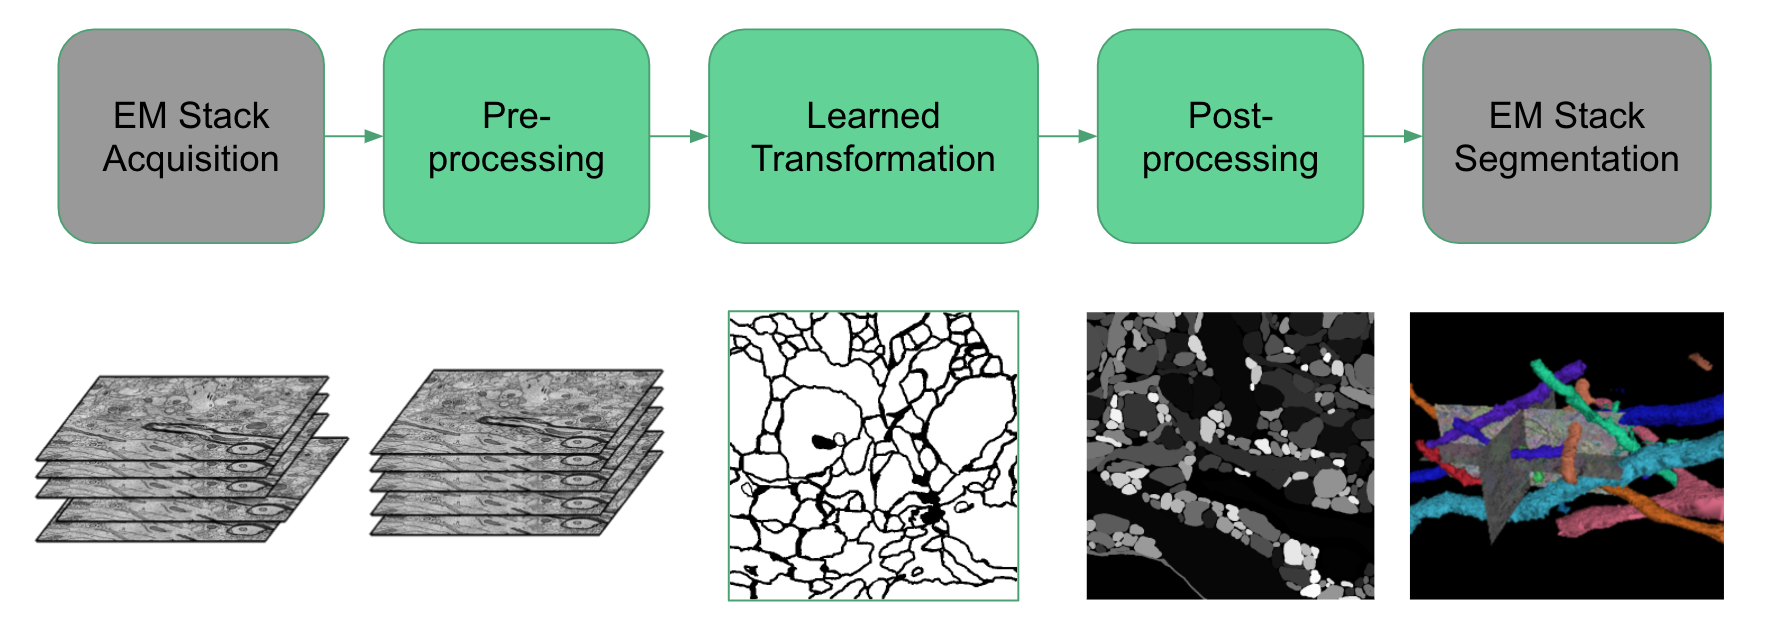
\includegraphics[width=\textwidth]{img/seg_pipeline.png}
\caption[A general outline of the EM segmentation pipeline]{A general outline of the EM segmentation pipeline. The lower set of images represent intermediate stages that the data takes on during processing. In this example, the images are first acquired through some sort of electron microscopy technique (typically ssTEM). Second, they undergo preprocessing, which is primarily realignment of slices that were disrupted in the imaging process. Third, a learned transform is applied, which in this case transforms the stack of images into an affinity map. Fourth, postprocessing is applied, which in this stage is computing an actual segmentation from the predicted affinities. Fifth, geometric segmentation is inferred from the pixel segmentation, and the data is ready for use in a downstream task. }
\label{fig:segmentation_pipeline}
\end{figure}

\subsection{Image Acquisition}
Given a physical volume of neural tissue, the first task in inferring tissue structure is to acquire some sort of digital representation of this tissue. While there are many techniques available for imaging biological tissue (e.g. light microscopy, electron microscopy, radiography, magnetic resonance imaging), typically the only way to acquire a representation of cell-level structures is by using a tunnelling electron microscope (TEM)\cite{Mielanczyk2015}. Before imaging, samples undergo considerable preparation: typically, they are embedded in a rigid medium that will allow them to be sliced with minimal distortion; additionally some sort of stain is applied to the tissue that affects the electrical properties of different biological structures, allowing for high-contrast imaging. The result is a set of slices of neural tissue, 30-50nm thick, that can be independently imaged in the TEM. When positional order from slicing is combined with the raw image data (which takes the form of grey-scale images, as opposed to RGB or CMYK images), each individual value can be treated as a voxel, since it is indexed by three orthogonal coordinates. Important to note is that these voxels are anisotropic, meaning that they are larger in the z-dimension than they are in the x-y dimension. This introduces a computational complexity that can somewhat be compensated for at later stages of the pipeline.

Although the actual performance of this physical imaging process is far ouside the scope of this thesis, we mention the physical steps involved because the methods used in preparing and imaging biological slices have immediate consequences on the quality of the data that is fed into stages of the pipeline in which we are primarily interested. Because the imaging process is physical and involves structures at nano-scale, physical preparation of the sample can introduce various defects into the slices that show up in resulting images. The staining process, for instance, can inconsistently vary contrast throughout an image, and can produce large dark blotches in an image. The slicing procedure can create tears and folds in tissue, which manifest as discontinuities in the images, and can even physically translate slices hundreds of nanometers. And since neural tissue naturally contains significant quantities of water, samples are prone to dry inconsistently, resulting in elastic warping of cell-level structures (like a rubber sheet that has local stretching). Visual examples of some of these artifacts can be found in Figure \ref{fig:imaging_errors}.

\begin{figure}
\centering
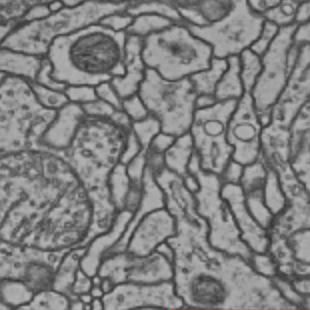
\includegraphics[width=0.3\textwidth]{img/normal_example.png}
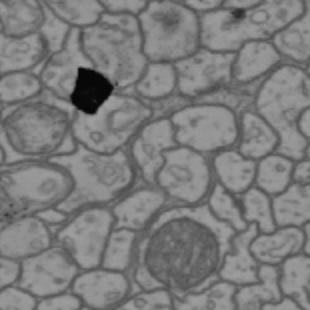
\includegraphics[width=0.3\textwidth]{img/stain_error.png}
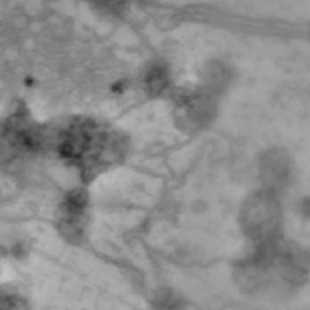
\includegraphics[width=0.3\textwidth]{img/blurred_example.png}
\caption[Examples of defects in the imaging process.]{Examples of defects in the imaging process. Left: a properly stained and imaged segment. Center: a slice where inconsistent staining or another artifact has left a large dark spot on the image. Right: a slice that was prepared in such a way that the microscope couldn't produce a sharp image, either during slicing or focusing.}
\label{fig:imaging_errors}
\end{figure}

These deformations caused by the imaging process can have drastic implications in the performance of later stages of the pipeline, especially when those stages aren't explicitly corrected for. We noticed that even slight misalignments in image data caused ultimate segmentation performance to noticably suffer. Later in the pipeline we will explore various techniques that can be used to make the pipeline more robust to these inevitable imaging defects.

\subsection{Preprocessing}
Once volume data is acquired, data usually will undergo any of several preprocessing techniques to prepare it for later stages of the pipeline. The scope of preprocessing and types of data transformations performed vary depending on the robustness of later stages of the pipeline, as well as requirements on the output of the segmentation pipeline. Preprocessing is generally treated as distinct from subsequent stages of the pipeline because the transformations often keep the data in the same domain of values, and maintain the data representation. In other words, both the input and the output of preprocessing take the form of stacked EM images. Typically, preprocessing will include some form of image adjustment and stack realignment.

Image adjustment can be as simple as altering the contrast on individual images, or making contrast uniform across the entire stack. While these adjustments will typically improve segmentation results, most modern deep learning techniques (which are liberally used in the subsequent pipeline stage) are easily trained to be quite robust with respect to level differences between images, so a rigorous exploration of image adjustment techniques would likely yield marginal gains in accuracy.\footnote{Training speed, however, could potentially see significant improvements, as a neural net would have to learn fewer functions if its input were more uniform} 

The same cannot be said for image alignment. The defects and imprecisions introduced in the actual imaging process can severly impact segmentation performance, particularly because they introduce three-dimensional discontinuities that make it difficult for many neural networks to trace continuous segments across slices. Thus, automatic stack alignment is an active area of research.

At its heart, the alignment problem is one of misrepresentative data. Ideally we would like each 'voxel' to spatially correspond to a true volume in the sample, and for a voxel's position in the the data to correspond to its true position within the greater sample. The defects in the imaging process taint this mapping, and we are left with a dataset that, when taken literally, misrepresents the physical volume from which it was derived. Thus, the task of realignment is to take this noisy data and distort it in some way so that it more accurately corresponds to the original volume.

While there are many theoretical ways of registering two images (registration here means alignment and distortion so that their features align accurately), most modern methods rely on establishing points of correspondence between two or more images, and distoring the images such that those points of correspondence end up at the same x-y coordinate in all images. It is generally believed that, given a high enough density of true correspondences throughout a stack, one can transform the data into a form that is pixel-for-pixel accurate with respect to the actual cellular structure of a sample.\footnote{Intuitively, this makes sense, since structures within cells are physically connected, our notion of correspondence is essentially a description of how these structures are physically connected.} The transformations themselves can be parameterized as elastic transforms, which provide discrete interpolation for all voxels not labeled as correspondences.

The problem, then, lies in actually determining these correspondences with high accuracy and high enough density for sample-accurate registration. One popular tool for achieving rough correspondences is \texttt{TrakEM2}, which provides functionality for registering generic images using a combination of the Scale Invariant Feature Transform (SIFT) and a global optimization \cite{Lowe1999}. This algorithm uses no learned or otherwise domain-specific knowledge, and is widely used across computer vision applications to stitch arbitrary images together. This process is sufficient for establishing rough correspondences, but the noisy and varied nature of cellular structures means that, without any more domain-specific correspondence labeling the resulting image registration on a moderately distorted dataset will likely not result in transformations that are smooth or accurate.

The Seung Lab's current realignment techniques attempt to use domain-specific techniques to achieve correspondence. These techniques are typically hand-designed filters that draw on domain knowledge of the consitution of EM slices of neural tissue, and require a non-trivial amount of hand-tuning when applied. To compute a realignment, first a sparse set of correspondences are made at the macro level, and a rough realignment is iterateively computed (the rationale being that iteratively computing many fine realignments has slow convergence and is computationally infeasable). Following this rough realignment, a much more granular set of correspondences are computed, and the stack is iteratively deformed a small number of times to compute a smooth, converged registration. This technique is quite effective, and leads to near-perfect registration, but requires a substantial amount of trained human input to determine both the parameters for the various correspondence filters and to correct obviously incorrect correspondences.

A more desirable approach would be to use machine learning to train a large set of filters (more specific ones than humans could compute) to predict correspondence at different levels of granularity. This is an active area of research within the Seung Lab. Alternatively, machine learning could be used to learn the actual parameters for a piecewise affine or elastic transform, rather than learn filters to predict corresponence, although as we demonstrate in Chapter 5 this is potentially quite difficult. 

Again, it is worth noting that failures in preprocessing to compensate for errors in the imaging stage - as well as new artifacts introduced in the preprocessing stage - will be propagated through the remainder of the pipeline, and can only have a negative or neutral impact on segmentation performance.

\subsection{Image Transformation}
The image transformation stage of the segmentation pipeline can loosely be defined as any set of transformations that compute a representation of the sample that is different in kind from a set of aligned images. In the case of most of the models discussed in this paper, the image transformation stage converts a stack of EM images into a 3D pixel-wise affinity map, where the labels at each pixel represent the probability that that pixel is in the same cellular body as the adjacent pixel in the x, y, and z direction. For other segmentation schemes, like Google's Flood-Filling architecture, the transformation output is a direct segmentation. 

This stage is perhaps the most well-explored in the pipeline for neural segmentation. While in the past hand-crafted or generic techniques were used in this stage to some degree of success (i.e. selective thresholding, hand-crafted filters, etc), most state-of-the-art techniques utilize some sort of machine learning scheme to learn the output representation, usually a neural net architecture that utilizes many successive convolutions to predict each pixel (or a small patch) of the output segmentation. These pixel/patch predictions can be stitched together to make a prediction on a whole stack. These ML approaches are typically supervised, and rely on using large datasets annotated with segmentations for training. Thus, as in most deep learning applications, the size and diversity of the training set is one of the most important factors in maximizing the generalization performance of this stage of the pipeline.

Because large, high-quality, labeled EM datasets are hard to come by (see the second sentence of this thesis), most researchers will take a reasonably-sized dataset and randomly apply data augmentations that make the data look like fresh data, thus artificially expanding the size of the dataset. These augmentation techniqes can broadly categorized as either affine transforms or elastic transforms. Specifically, researcher will usually introduce some sort of scaling, rotation, shearing, and elastic warping to both the image stack and the labels. These techniques have an enormous impact on accuracy and generalization - empirical evidence of this  is provided in Chapter 3.

The specific network architectures that are used in this stage of the pipeline are quite varied. We will describe the general classes of architectures relevant to our exploration here, and will revisit specific architectures we used later in this paper. Additionally, it is worth noting that elements of various architectures listed below can be combined (i.e. adding residual connections to standard convolutional nets.)

\subsubsection{Standard Convolutional Networks}

\begin{figure}
\centering
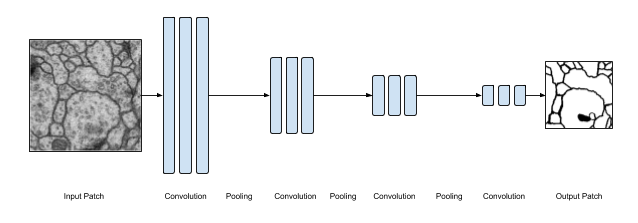
\includegraphics[width=\textwidth]{img/Fully_Convolutional_Network.png}
\caption[A prototypical Fully Convolutional Neural Network]{A prototypical Fully Convolutional Network, with successive convolutional layers followed by pooling layers. Depending on the types of convolution layers, the size of the input may be much larger than the size of the output, implying that the field of view for each pixel in the output could be greater than 1.}
\label{fig:fully_conv_net}
\end{figure}

The most conceptually simple type of network that is used is the standard convolutional network, depicted in Figure \ref{fig:fully_conv_net}. Standard convolutional nets typically involve several successive convolutions with small filters (e.g 3x3x3 filters) that perform either 'valid' or 'same' convolutions, which are differentiated by the size of the output of the convolution. After each convolution, a nonlinearity (e.g. ReLU) is applied, and every so often pooling layers are interspersed to alter the scale of the underlying feature maps. At the end of these alternating convolutions and poolings is a prediction, often the output of a sigmoid, that predicts a single pixel or patch of boundaries (or affinities, in the 3D case). Depending on the number of convolutions and poolings, the output pixel is determined by pixels within a certain field of view in the input image - that is, if one were to mathematically unroll the convolutions and poolings, only a certain number of pixels in the input image would be used to compute the prediction in the output image. In the N4 architecture applied in 2 dimensions, for instance, each pixel in the output prediction is influenced by pixels in a bounding box of 96x96 pixels. Architectures that are primarily Standard Convolutional Networks include N4 (2-dimensional), VD2D (2-dimensional), and VD2D-3D (3-dimensional)\cite{Cirean,Lee}.

\subsubsection{U-Net}

\begin{figure}
\centering
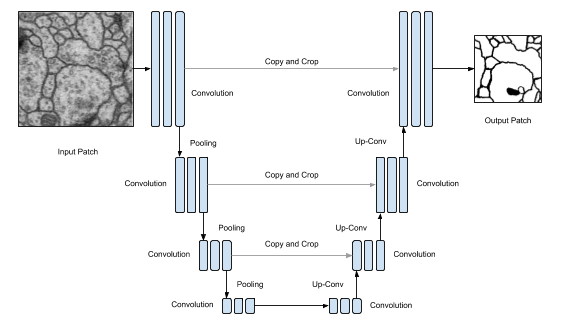
\includegraphics[width=\textwidth]{img/U_Net.png}
\caption[A prototypical U-Net]{A prototypical U-Net, with successive convolutional layers followed by pooling layers on the downward pass, and then successive convolutional layers followed by up-convolutions on the upward pass. Notice how the inputs to each convolution after an up-convolution also takes as input the output of the last convolution of the corresponding layer in the downward pass.}
\label{fig:u_net}
\end{figure}

U-Net style architectures closely resemble autoencoders, in that they compress a representation of an input using convolutions and poolings, and then decompress that representation using convolutions and up-convolutions.  However, instead of trying to predict a perfect reconstruction of the input, the U-Net architeture attempts to reconstruct boundaries/affinities for the input image. One key feature of U-Nets is the symetrical use of skip connections - for every convolutional layer on the compressive (downward) pass, the output of those convolutions is added to the input of corresponding convolutional layers on the decompressive (upward) pass. This serves to force the net to quickly learn a set of affinities that look like the input. Much like Standard Convolutional Networks, every pixel in the output patch of a U-Net architecture can be affected by pixels in a certain field of view in the original input - modifying this field of view can often modify the quality of the results. Empirically, the predictions of U-Net architectures tend to be significantly smoother than fully convolutional architectures (although they may not be more accurate). A prototypical U-Net can be seen in Figure \ref{fig:u_net}. Architectures that are primarily based on the U-Net style are the original U-Net (2 dimensional), 3D U-Net (3 dimensional), and V-Net. SegNet also resembles the U-Net architecture, in drawing inspiration from the autoencoder paradigm\cite{Ronneberger2015,Cicek2016,Milletari2016,Badrinarayanan2015}.

\subsubsection{Residual Nets}

\begin{figure}
\centering
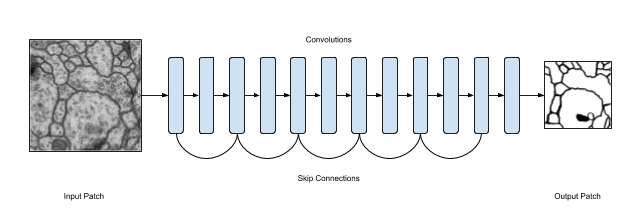
\includegraphics[width=\textwidth]{img/Residual_Network.png}
\caption[A prototypical Residual Net]{A prototypical Residual Net, which has a similar structure to the Fully Convolutional Network. The major difference is the skip connections - the residual connections - are added right before the nonlinearity but after a convolution. Residual connections can be added to other architectures to achieve some of the properties of this network.}
\label{fig:residual_net}
\end{figure}

Residual Networks draw on a similar idea as U-Net, in that convolutional layers should be able to directly influence layers that do not directly follow them in the architecture\cite{He2015}. As shown in Figure \ref{fig:residual_net}, Residual Nets add skip connections that jump over one (or more) sets of convolutions. Deeper nets are, in general, quite difficult to train, and the use of residual connections often increases the speed of training for deeper architectures.

\subsubsection{Flood-Filling Networks}
Flood-Filling Networks (FFNs) take a different approach to the prediction task. Rather than predict whether a pixel in the output is a boundary or not on a given input, FFNs are given an input patch and an x-y coordinate, and output a pixel mask for that patch that represents whether a pixel in the output is in the same body as the input x-y coordinate\cite{Januszewski2016}. If a particular object is sampled such that the output patches completely cover the object, a full segmentation of that object can be achieved (successive sample patches are chosen by a recurrent neural net (RNN)). Typically, this map is predicted with several convolutions, although architectures are varied. While we will not explore FFNs any further, as they are outside the scope of the research presented in this paper, they are noteworthy in that directly predict segmentation, rather than an intermediate (and thus require substantially less postprocessing than other menthods).


\subsubsection{Typical Errors}
The errors made by neural networks in the Image Transformation stage (and ultimately affect the accuracy of the resulting segmentation) tend to fall into several categories: split errors, merge errors, and incorrect object shaping. These errors are somewhat self-explanatory. Split errors occur when networks predict intermediates that, when converted into a segmentation, incorrectly split a body into two distinct segments when it should be one. Similarly, merge errors occur when two distinct objects are labeled as the same object. Incorrect object shaping occurs when the output of the network incorrectly predicts boundaries that may not necessarily cause merge or split errors, but simply predict boundaries that are too thick or otherwise encroach on the true shape of the object. These sorts of errors can be mitigated either by altering network architecture, or through postprocessing.

Important to note is the fact that the quality of the input data has a huge effect on the quality of the output data. While data augmentations during training can help networks compensate for misaligned data, generally inputs that are well-aligned will result in significantly better predictions than those that are poorly aligned. It is difficult to completely correct for this at the Image Transformation stage, which is why we stress the importance of the Preprocessing stage in preparing data well for segmentation.

\subsection{Postprocessing}
Once the EM stack data has been transformed into an intermediate form (i.e. boundaries/affinities, or segementation in the case of Flood-Filling Networks), postprocessing is often applied. Postprocessing can take on many forms, but often involve using the intermediate form to prepare a segmentation. Given a boundary/affinity map, there are many different ways to infer a segmentation of an image. However, we will discuss two methods that are used in the Seung Lab to process boundaries/affinities into segmentations.

\subsubsection{Watershed Transform}
The Watershed Transform is a standard computer vision algorithm for segmenting images. Given an affinity graph, the algorithm treats the values of affinities as energy values, which is analogous to the height of land in a geographical landscape. Since pixels that belong to the same body have high affinity, the topological high-points will be the bodies themselves, and the valleys will be the boundaries between bodies. The watershed variant used in the Seung Lab identifies the plateaus (representing distinct objects) and uses those identified plateaus to inform where to place basins for the classical watershed algorithm. The algorithm then floods basins based on a set of supplied parameters. This allows a distinct labeling of all pixels in the image, where pixels in the same basin are given the same label. All bodies that are too small to actually be distinct bodies are merged greedily. It is at this stage where merge/split errors often manifest, since two basins could be split or merged if there are discontinuities in an affinity boundary, or if non-cell-wall affinites are too high. Selecting appropriate parameters for this task is paramount in finding a good segmentation, and is typically performed empirically for a given dataset.

\subsubsection{Mean Affinity Agglomeration}
One way to mitigate some of the merge/split errors that arise from the Watershed Transform's intolerence of slightly imprecise affinities is to artificially heal the imperfections in boundaries that are generally correct. Mean Affinity Agglomeration (MAA) is one way to do this. MAA iterates over boundaries between segmented objects and greedily merges or splits them based on the mean affinity along the boundary. In this way, inconsistent boundaries predicted by the Image Transform stage can be healed.

\subsection{Segmentation/Downstream Processing}
Once postprocessing has occurred, the data is now in a completely segmented form. The segmentation can then be used for downstream tasks. Theoretical applications of segmentation include labeling different cells by their type, generating weighted directed graphs that represent connections between neurons, and determining characteristics of neurons in different types of tissue.
\chapter{The \texttt{DeepSeg} Framework}
So far we have discussed the theoretical computational concepts that underpin the EM segmentation pipeline, and realized that there are many nuanced computational steps that flow into one another during the segmentation of an EM volume. Given the algorithmic intricacy of the computational tasks, it stands to reason that any software implementation of the computational tasks will be large and complex. Conventional wisdom holds that a large and complicated software package is anathema to a researcher attempting to experiment with, augment, and improve upon the techniques implemented in that software package. Repeatability of experiments is also critical to a researcher retaining his or her sanity, so a pipeline that is completely automatic and is completely specified by a consolidated set of parameters is critical.

As our research group started building and modifying software to experiment with different stages of the segmentation pipeline, it became painfully obvious that as our codebase grew in size and complexity, it was becoming increasingly difficult to alter the software without making major modifications across the codebase. So, in order to avert collective anguish we decided to design a framework - which we tentatively have named \texttt{DeepSeg} - with the following set of goals:

\begin{itemize}
	\item to create a set of abstractions and interfaces that allow researchers to modify or swap-out different components with minimal software-level impacts on the functionality of other portions of the pipeline.
	\item to define abstractions for model development that are succinct and use domain-knowledge about the problem to automatically connect to sampling mechanisms during the training process. 
	\item to be completely portable accross different machines and host environments, and to automatically integrate with installed GPU hardware for training acceleration.
\end{itemize}

On the technical level, the DeepSeg is written in \texttt{Python} (with some \texttt{Julia} and \texttt{C++} tools), and uses the \texttt{NumPy} package to represent and manipulate data throughout the pipeline. All of the machine-learning components, particularly for model definition and training, are built on top of the TensorFlow, Google's popular, open-source deep learning framework\cite{Abadi}. This was chosen because of its ease of use with \texttt{Python}, its flexibility, and its automatic integration with GPUs via \texttt{CUDA}.

In the following subsections, we will describe the abstractions introduced in the DeepSeg framework, and some of the underlying implementation details of these abstractions.

\section{Overview}

The driving concept behind the design of the system is being able to specify the entire pipeline in one place. This includes specifying all dataset handling, preprocessing, image transformation, and postprocessing procedures and parameters. Additionally, for any components that require learning or optimization, training parameters and inference specification are explicitly required. Because every non-parameter component in the specified pipeline must adhere to specific interfaces (i.e. dataset samplers must provide data samples of a specific size), components can be freely swapped out in the specification with the knowledge not only that the pipeline will execute, but the only meaningful difference in execution will occur at the altered component.

In terms of functionality, the framework provides both training and inference for a specified pipeline. The training process automatically hooks into \texttt{TensorBoard}, the \texttt{TensorFlow} training visualization tool, in order to monitor training progress. The pipeline can automatically load trained models for inference tasks, and supports exporting into formats accepted by various EM segmentation competitions.

\section{Pipeline Specification}

A pipeline can be completely specified with a set of parameter classes:

\begin{itemize}
\item \texttt{PipelineConfig}: The main configuration class, which contains all other sets of parameters, as well as which models are used, where to find datafiles, and where to save results.
\item \texttt{TrainingParams}: The set of parameters used in a training process, including learning rate, optimizer, patch sample sizes, and batch sizes.
\item \texttt{AugmentationConfig}: A set of booleans determining which augmentations to use when sampling the dataset.
\item \texttt{InferenceParams}: The set of parameters used when performing inference, including how to assemble predictions on large images from smaller predictions.
\end{itemize}

A \texttt{PipelineConfig} object is passed to the \texttt{Learner} class, where all the relevant componenets are connected.

\section{Handling Diverse Datasets and Label Types}

Currently, the framework supports several different datasets out of the box: the ISBI 2012 EM boundary-detection dataset, the ISBI 2013 SNEMI3D EM segmentation dataset, and all the datasets provided by the CREMI 2016 EM segmentation challenge. Prediction preparation tools are available to reformat the predictions on test sets for submission to their respective leaderboards. The framework also supports arbitrary EM datasets of any reasonable size,\footnote{Any dataset that fits in RAM.} and supports label inputs as segmentations, boundaries, 2D affinities, and 3D affinities.

Raw datasets are wrapped by classes that implement the \texttt{Dataset} interface (i.e. \texttt{CREMIDataset}, \texttt{SNEMI3DDataset}, and \texttt{ISBIDataset}).


\section{Dataset Sampling}

The framework provides several different modes for sampling a specified dataset during training or inference. For training, random samples of arbitrary shape can be sampled, to which specified augmentations are applied. For inference, entire validation and test sets can be sampled in formats that are appropration for feeding into the pipeline.

\subsection{Augmentation}

The framework supports several type of random augmentation:

\begin{itemize}
	\item Rotation: the entire stack can be rotated by a random angle.
	\item Flipping: the entire stack can be randomly mirrored along the x, y, or z axis.
	\item Blurring: individual slices within a stack can be arbitrarily blurred.
	\item Warping: individual slices can be warped via elastic deformation, to simulate data that is structurally different from the underlying dataset.
\end{itemize}

All augmentations are parameterized within certain bounds. Additional augmentations could theoretically be added to the pipeline with ease.

Sampling is primarily configured and executed by the \texttt{EMSampler} class.

\subsection{Parallelization}

For multi-core training environments, the framework parallelizes the sampling procedure, executing data sampling on multiple cores and adding the samples to a data queue, which can be sampled at each training step. This considerably speeds up training time when using GPUs, especially when the timing of the augmentation procedure is non negligible with respect to the timing of an optimization step.

\section{Preprocessing}

The framework enables the specification of preprocessing procedures to be executed before data flows into the Image Transformation stage of the pipeline. Currently the type of preprocessing procedures is limited to realignment using Spatial Transformers (anything that implements the \texttt{SpatialTransformer} interface) and standardization (a.k.a. whitening) of data, but it would be simple to implement additional preprocessing functionality.

\section{Image Transformation}

The framework allows clients to specify which type of image transformation should be included in the pipeline. Currently, the only types of image transformations that are directly implemented in the framework are variants of the Fully Convolutional Net and the U-Net\footnote{RNN-based Flood-Filling Networks may be available soon.}. In general, the Image Transform stage must take a 5-dimensional \texttt{Tensor} (the fundamental datastructure used in \texttt{TensorFlow}) with a shape of [batch-size, z-size, y-size, x-size, num-channels], and outputs a 5-dimensional \texttt{Tensor} with a shape of [batch-size, z-size, y-size, x-size, [1-3]] containing the predictions on the input data. The Image Transform must specify a \texttt{predict} function for inference.

\subsection{Model Definition}

There are only two broad classes of models currently supported: \texttt{ConvNet}(Fully Convolutional Nets), and \texttt{UNet}(U-Nets). However, the framework provides a set of primitives for each classes that allow for concise construction of nets with arbitrary structure, so long as they fit within the general paradigm of these two model types. These architectures are specified by both the \texttt{ConvArchitecture} and the \texttt{UNetArchitecture} classes, and are fed as parameters to the \texttt{ConvNet} and \texttt{UNet} classes for construction and automatic integration into the pipeline.

Particularly useful is that both classes of models automatically calculate the field-of-view of the models, and expose both the input and output shape to the pipeline so that at training time and inference time no extra specification or \texttt{Tensor}-wrangling must occur outside of the models. This means that to modify the architecture of a net, one need only change its respective \texttt{Architecture} specification, and nothing else. An example of an architecture specifcation for the 2-D N4 archetecture can be found below:

\begin{lstlisting}
N4 = ConvArchitecture(
    model_name='n4',
    output_mode=BOUNDARIES,
    layers=[
        Conv2DLayer(filter_size=4, n_feature_maps=48, activation_fn=tf.nn.relu, is_valid=True),
        Pool2DLayer(filter_size=2),
        Conv2DLayer(filter_size=5, n_feature_maps=48, activation_fn=tf.nn.relu, is_valid=True),
        Pool2DLayer(filter_size=2),
        Conv2DLayer(filter_size=4, n_feature_maps=48, activation_fn=tf.nn.relu, is_valid=True),
        Pool2DLayer(filter_size=2),
        Conv2DLayer(filter_size=4, n_feature_maps=48, activation_fn=tf.nn.relu, is_valid=True),
        Pool2DLayer(filter_size=2),
        Conv2DLayer(filter_size=3, n_feature_maps=200, activation_fn=tf.nn.relu, is_valid=True),
        Conv2DLayer(filter_size=1, n_feature_maps=1, is_valid=True),
    ]
)
\end{lstlisting}

\subsection{Model Training}

Model training primarily occurs through the \texttt{Learner} class, which creates an optimizer based on a model's specified loss function (typically cross entropy), as well as various parameters specified in \texttt{TrainingParams}. Every step, the \texttt{Learner} feeds a training example from the queue into the model, runs the optimizer for one update step, and executes any number of user-specified \texttt{Hook}s. These hooks will execute every $N$ steps, where $N$ is specified by the user in the hook constructor. Hooks provided include:

\begin{itemize}
	\item \texttt{LossHook}: Report the loss for the model to \texttt{TensorBoard} every $N$ steps.
	\item \texttt{ValidationHook}: Run inference on the validation set every $N$ steps, and write both validation scores and image predictions to \texttt{TensorBoard}.
	\item \texttt{ModelSaverHook}: Save the model variables to disk every $N$steps, so that the model can be reloaded for inference.
	\item \texttt{HistogramHook}: Write distributions of the values of parameters for each \texttt{TensorFlow} variable to \texttt{TensorBoard} every $N$ steps.
	\item \texttt{LayerVisualizationHook}: Write visualizations of the various feature maps for different convolutional layers to \texttt{TensorBoard} every $N$ steps.
\end{itemize}

\section{Postprocessing}

Much like the preprocessing stage, the postprocessing stage of the pipeline allows for arbitrary transformations of the output of the Image Transformation stage. The only two transforms currently included in the framework are:

\begin{itemize}
	\item Watershed: Given a set of specified parameters, convert a dataset annotated with affinities to a segmentation of the dataset. The current version is implemented in Julia.
	\item Mean Affinity Agglomeration: Given a segmentation and a set of affinities, greedily merge or split regions based on the affinity continuity along borders of the regions. The current version is also implemented in Julia.
\end{itemize}

\section{Ensembling}

The framework also enables the use of various ensembling techniques both at training time and at inference time through the \texttt{EnsembleLearner} class. This class allows a group of models to be trained simultaneously, and upon the completion of this training, an ensembling technique can be applied to their outputs for prediction. This ensembling technique can be any arbitrary ensembling method, including learned ensembling techniques that train on the outputs of various models. Currently the framework supports the following ensembling methods:

\begin{itemize}
	\item \texttt{ModelAverager}: Average the output of several different models. If multiple copies of the same net are trained independently, averaging the outputs reduces the variance of predictions and leads to higher accuracy.
\end{itemize}

\section{GPU Acceleration and Portability}

Paramount in modern deep learning training is GPU Acceleration. In our experiments, using a GPU accelerated training speeds by factors of 100 or more, which was indispensible in the experimentation process. Because the entire pipeline sits on top of a \texttt{TensorFlow} backend, and \texttt{TensorFlow} automatically optimizes its own internal processing graph for use on GPUs that support \texttt{CUDA}, our framework is GPU-enabled by default.

Because our group did not have a dedicated set of GPU hardware at the beginning of the project, we decided to use the containerization platform Docker, along with some NVIDIA plugins, to enable GPU training on any Linux machine with a GPU. By creating a Docker container that has the entire framework pre-installed, training and inference can be run on any machine that has access to a GPU with minimal setup.


\chapter{2D Segmentation}

In this chapter, we establish the task of 2D Segmentation of EM images, attempt to train models that perform well on this task, and evaluate our results. The purpose of these experiments is not so much to achieve state-of-the-art performance on the task, but to examine the effect that increasing training data quality and reducing variance in predictions has on model performance.

\section{Task Definition}

2D Segmentation involves taking a single 2D slice of EM tissue and segmenting it into its constituent cells. Compared to 3D segmentation, this is a simple task, but will still allow us to show the properties of different models on EM data. To achieve segmentation, we will train models that predict boundaries of cells, and then use a Watershed algorithm to segment based on those boundary predictions.

The problem statement for 2D Boundary detection is such: given a 2-dimensional single-channel (i.e. greyscale) image of neural tissue taken with an electron microscope, produce an image that labels the boundaries of all the distinct cells in the image. An example of this boundary-detection task can be found in Figure \ref{fig:isbi_example}. This task is made somewhat more difficult by the existence of organelles with well-defined borders, as well as blood vessels and structured interstitial tissue.

\begin{figure}
    \centering
	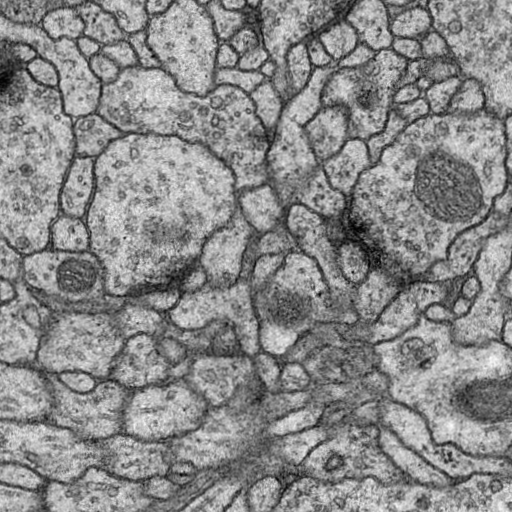
\includegraphics[width=0.33\textwidth]{img/isbi_raw_example}
	\hspace{1cm}
	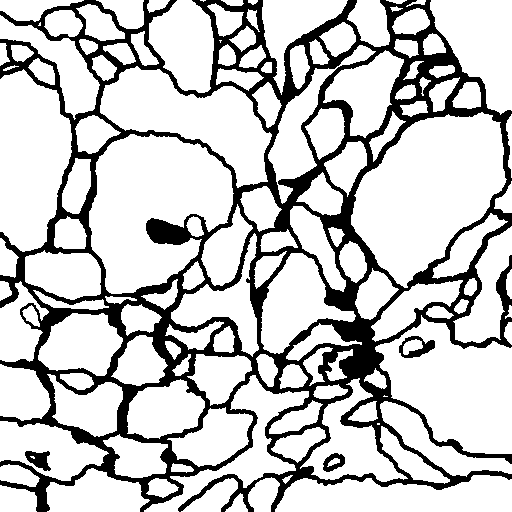
\includegraphics[width=0.33\textwidth]{img/isbi_label_example}
    \caption[An example of 2D boundary detection]{An example of 2D boundary detection. Left: the original image taken with an electron microscope. This particular example is neuron tissue taken from \textit{Droposphila melanogaster} in a dataset created for the ISBI 2012 EM segmentation challenge \cite{Arganda-Carreras2015}. The resolution of each pixel is 4nm x 4nm. Right: The ground truth boundaries corresponding to cell membranes in the input image, as labeled by human experts. The labels are binary values, although the actual border deliniation is somewhat arbitrary due to the fact that real applications of boundary detection are invariant to small differences in boundary shapes.}
    \label{fig:isbi_example}
\end{figure}

\section{Evaluation Metrics}

The two main evaluation metrics we will use for this task are Rand Error and Pixel Error. Formal definitions of both of these error metrics can be found in Appendix A. 

\begin{itemize}
\item \textbf{Rand Error}: We will use the Rand Error to determine whether or not the segmentation process correctly labels different cells as different objects. We will also look at the Rand Split Error and the Rand Merge Error, to see where the models inaccurately split and merge different regions.
\item \textbf{Pixel Error}: We will use the Pixel Error to gauge the efficacy of our models at predicting the intermediate boundary stage.
\end{itemize}

\section{Models}

We define two models - both closely resembling models from the literature -  with which we will run experiments:

\begin{itemize}
\item \textbf{N4}
\item \textbf{VD2D}
\end{itemize}

\section{Dataset}

\TODO{Talk about splits}

One prominent competition that evaluates performance on this sort of task is the International Symposium on Biomedical Imaging (ISBI) EM Segmentation Challenge, which has had active submission since 2012. The ISBI Challenge organizers provides a training set of EM images, along with a set of binary boundary maps. The challenge website describes the training data as \quotes{a set of 30 sections from a serial section Transmission Electron Microscopy (ssTEM) data set of the Drosophila first instar larva ventral nerve cord (VNC). The microcube measures 2 x 2 x 1.5 microns approx., with a resolution of 4x4x50 nm/pixel}\cite{Arganda-Carreras2015}. This resolution description implies that each pixel represents a 4x4nm patch on the surface of a slice, with each slice being 50nm thick. We build prediction systems using several different architectures, regularization methods, and data transformation techniques. We make several submissions to the leaderboard, ultimately scoring quite competitively.

\section{Training}

\section{Results}

\begin{table}
\centering
	\begin{tabular}{lllll}
\toprule
{} & Pixel Error & Rand - Full & Rand - Merge & Rand - Split \\
\midrule
N4 w/o aug   &    0.112204 &     0.65693 &     0.506545 &     0.934315 \\
N4           &   0.0827646 &    0.950296 &     0.933164 &     0.968069 \\
VD2D w/o aug &   0.0998995 &     0.80245 &     0.725266 &     0.898018 \\
VD2D         &   0.0842352 &    0.954286 &     0.976404 &     0.933148 \\
VD2D (x5)    &    0.083214 &    0.975745 &     0.985624 &     0.968843 \\
\bottomrule
\end{tabular}

	\caption[Results of 2D Segmentation]{The results of various architectures on the 2D Segmentation task. Notice that using data augmentation drastically improves the performance of the nets. Additionally, ensembling multiple instances of the best architecture produces the best Rand Score.}
	\label{tab:2d_results}
\end{table}

\begin{figure}
\centering
\textbf{Rand Index}
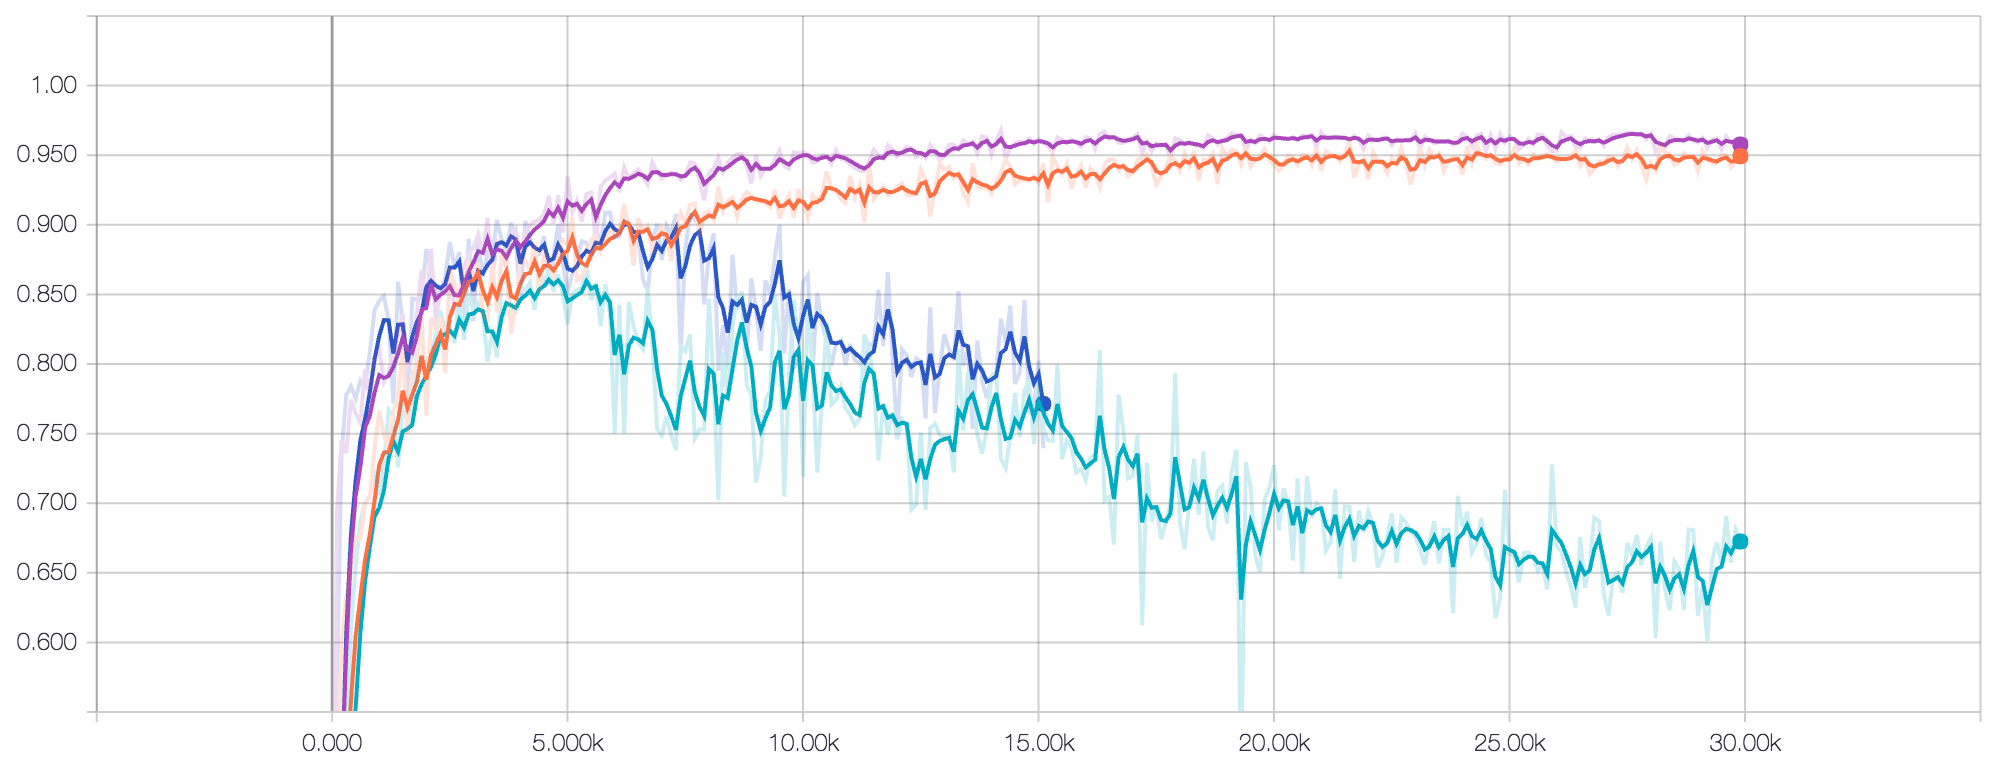
\includegraphics[width=\textwidth]{img/2d_rand.png} \\
\textbf{Pixel Error}
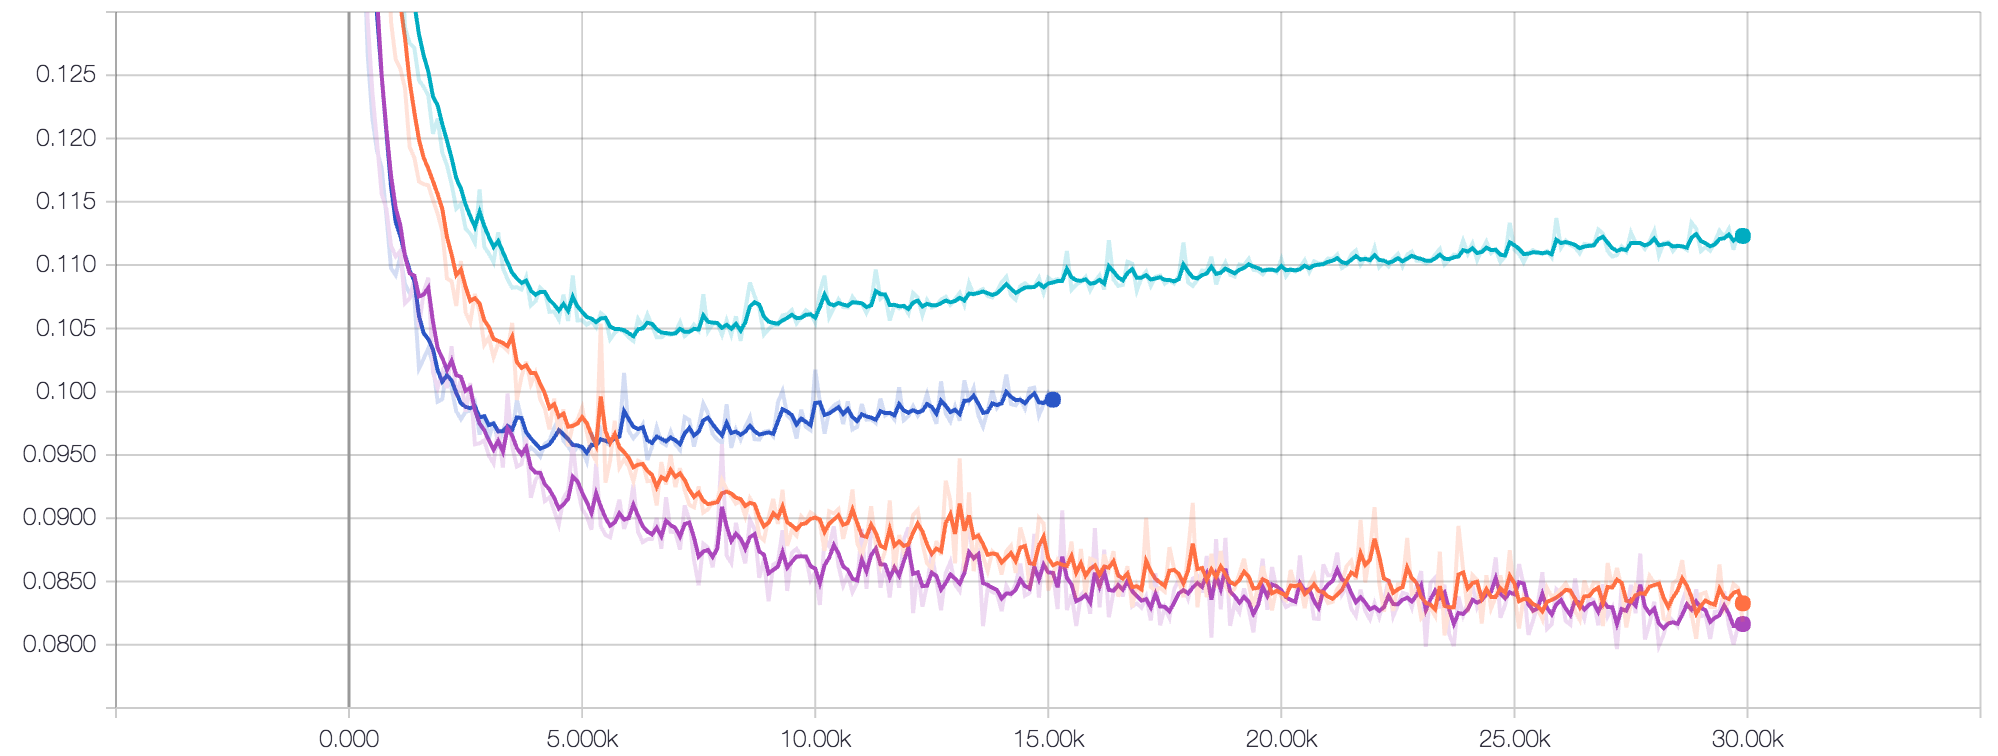
\includegraphics[width=\textwidth]{img/2d_pixel.png}
\label{fig:training_curves}
\caption[Training curves for 2D segmentation]{Training curves, smoothed, for 2D segmentation. Top: The full Rand scores on the validation set (from top: VD2D, N4, VD2D w/o augmentation, N4 w/o augmentation). Bottom: The pixel error on the validation set (from top: N4 w/o augmentation, VD2D w/o augmentation, N4, VD2D).}

\end{figure}

\section{Discussion}
\chapter{3D Segmentation}

In this chapter, we establish the task of 3D Segmentation of EM Images, attempt to train models that perform well on this task, and evaluate our results. The purpose of these experiments is not so much to achieve state-of-the-art performance on the task, but to examine the effect that increasing training data quality and reducing variance in predictions has on model performance.

\section{Task Definition}

The problem of 3D Segmentation is formulated as such: given a stack of 2-dimensional EM images generated that represent a 3-dimensional volume of tissue (i.e. the images were taken of successive physical slices of tissue), produce a segementation\footnote{A segmentation of an image or a stack of images is defined as producing a label for each pixel in the image or stack of images, where each unique label corresponds to a discrete object in the physical volume.} of the set of images that uniquely labels each discrete entity in the original volume. That is, if a tissue volume contains a neuron that passes vertically through several different slices, then the portions of each slice through which the neuron passes would be labeled with the same identifier. This problem is significantly more complicated than the boundary prediction problem stated before, because it requires an awareness of context in 3 dimensions, rather than 2. Additionally, most EM datasets are anisotropic, meaning that the resolution is not uniform in all directions (specifically, the z-direction perpendicular to the plane of each image is generally dilated). An example of a segmentation can be found in Figure \ref{fig:snemi3d_example}.

\begin{figure}[h]
    \centering
	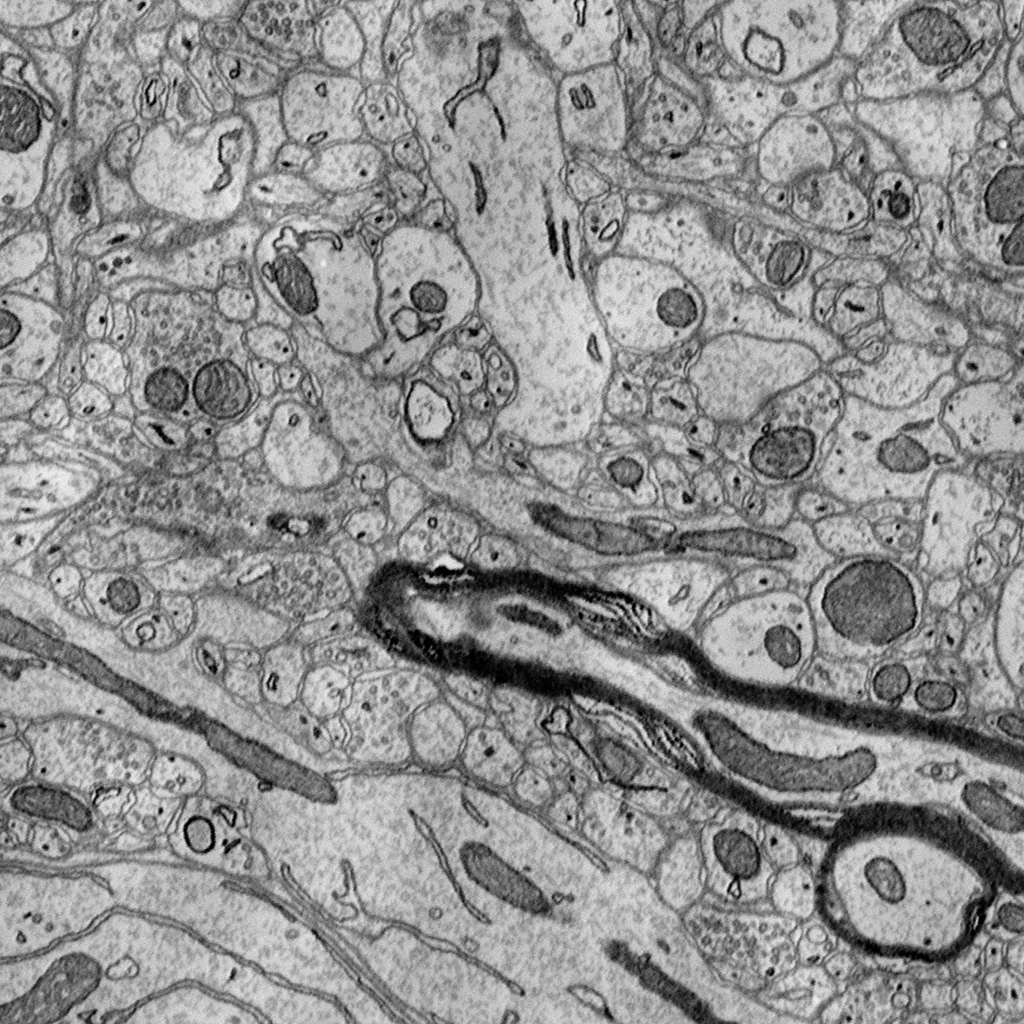
\includegraphics[width=0.33\textwidth]{img/snemi3d_raw_example}
	\hspace{1cm}
	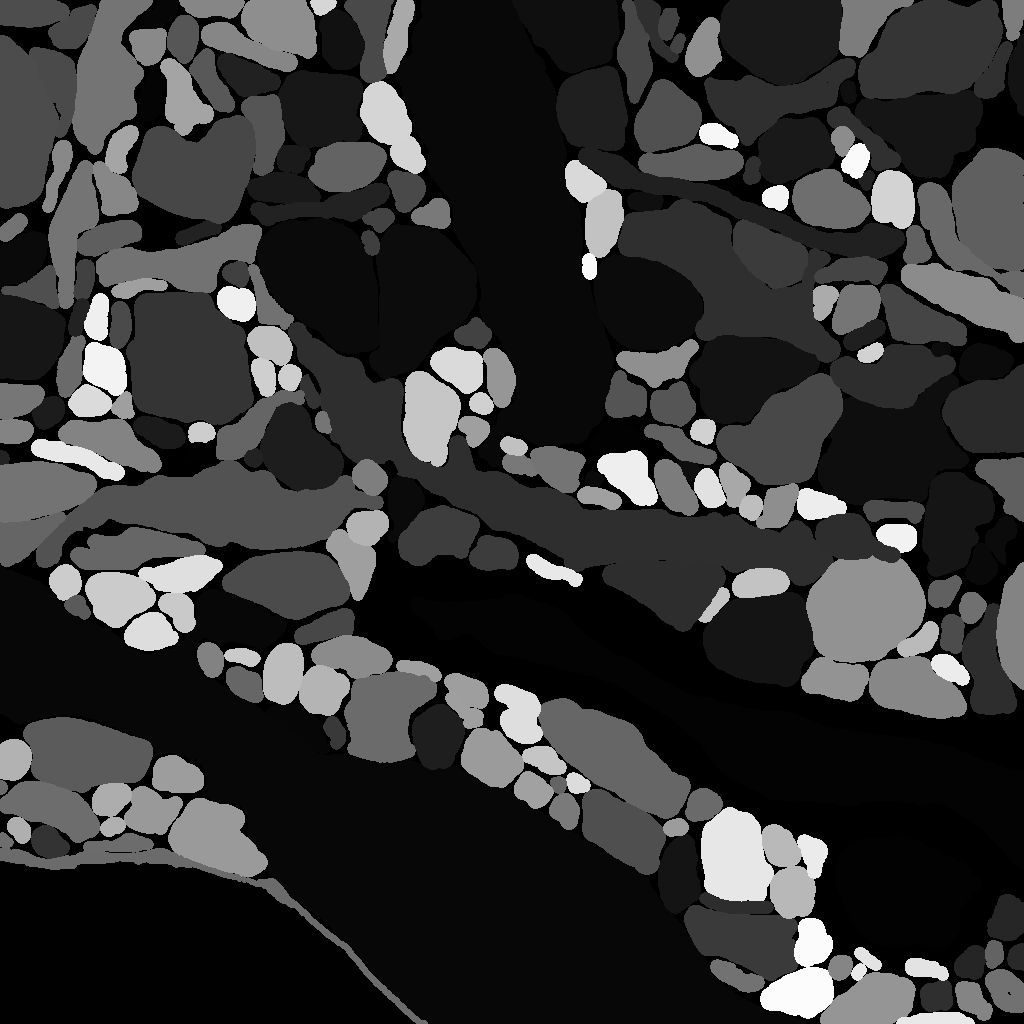
\includegraphics[width=0.33\textwidth]{img/snemi3d_label_example}
    \caption[An example of a 2D cross-section of a 3D segmentation]{An example of a 2D cross-section of a 3D segmentation. Left: one of the original images in a stack of images taken with an electron microscope. This particular example is neuron tissue taken from the common mouse in a dataset used in the ISBI 2013 EM segmentation challenge \cite{Kasthuri2015}. The resolution of each pixel is 6nm x 6nm, and each image represents a slice 30nm thick. Right: The ground truth segmentation corresponding to a segmentation of each individual object in the input image, as labeled by human experts. The labels are unique identifiers, although the border deliniation is somewhat arbitrary due to the fact that real applications of boundary detection are invariant to small differences in boundary shapes.}
    \label{fig:snemi3d_example}
\end{figure}

Trivially, the complexity of objects in 3 dimensions is potentially much greater than in two dimensions, so it makes sense that any learning method used to train a system that performs segmentation might be adept at certain types of volumetric data, and inept at others. To evaluate methods on different types of volumetric data, we selected two different challenges that provide us with samples of neural tissue that have different geometric properties, not only due to geometric differences in the underlying tissue but also because of differences in sample preparation techniques. These two challenges are the SNEMI3D Segmentation Challenge and the CREMI Segmentation Challenge.

\section{Evaluation Metrics}

Similar to the 2D Segmentation task, the two main evaluation metrics we will use for this task are Rand Score and Pixel Error. Formal definitions of both of these error metrics can be found in Appendix A. 

\begin{itemize}
\item \textbf{Rand Score}: We will use the Rand Score to determine whether or not the segmentation process correctly labels different cells as different objects. We will also look at the Rand Split Score and the Rand Merge Score, to see where the models inaccurately split and merge different regions.
\item \textbf{Pixel Error}: We will use the Pixel Error to gauge the efficacy of our models at predicting the intermediate boundary stage.
\end{itemize}

\section{Models}

We define two models for experimentation:

\begin{itemize}
	\item \textbf{VD2D-3D}: The VD2D-3D implemented for this experiment is close to the one published by Lee et. al.\cite{Lee}. It is a standard, fully-convolutional architecture that consists of two computational stages. The first stage of the net computes a series of 2D convolutions and poolings on each slice of a given sample stack, and the second stage computes a series of 3D convolutions and poolings on the entire stack. Intermediate nonlinearities are ReLU. Because the dataset is anisotropic, the effective field of view in the z direction is much smaller than in the x and y direction in terms of pixels, which is achieved through fewer z-dimensional poolings and smaller z-dimensional convolutions. The model predicts a set of 3 affinities (x, y, z) for each pixel. The effective field of view is a 85 pixel square in the x-y plane, and 7 pixels in the z direction.

	\begin{figure}
	\centering
	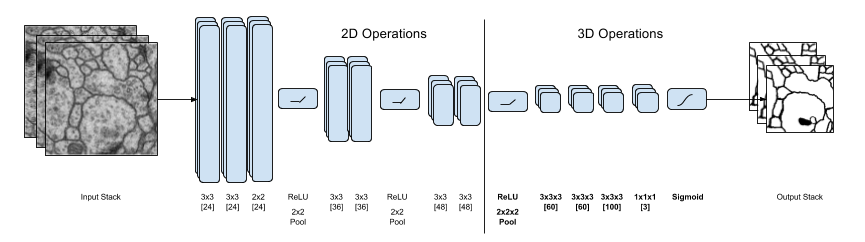
\includegraphics[width=\textwidth]{img/VD2D_3D.png}
	\caption{The VD2D-3D architecture for 3D Segmentation.}
	\label{fig:vd2d_3d}
	\end{figure}

	\item \textbf{UVR-Net}: The UVR-Net borrows concepts from the U-Net, V-Net, and Residual Nets, and is an architecture that all members of our group contributed to\cite{Ronneberger2015,He2015,Milletari2016,Cicek2016}. The structure consists of 4 "U Layers", which are pairs of down-convolutions and up-convolutions. The output of the down-convolutions skips across the net, and is concatenated to the input of the corresponding up-convolutional component (the number of feature maps of the first convolution in each "U Layer" is twice the subsequent ones). We add residual connections that skip the convolutions from the output of pooling layers, and add skip connections across the "U-Layer". After each convolution, we apply ReLU nonlinearities, except between convolutions and additions with residual connections. These modifications are all added to attempt to make the net learn first by predicting an output that looks similar to the input, and slowly eroding elements until an affinity map is left.

	\begin{figure}
	\centering
	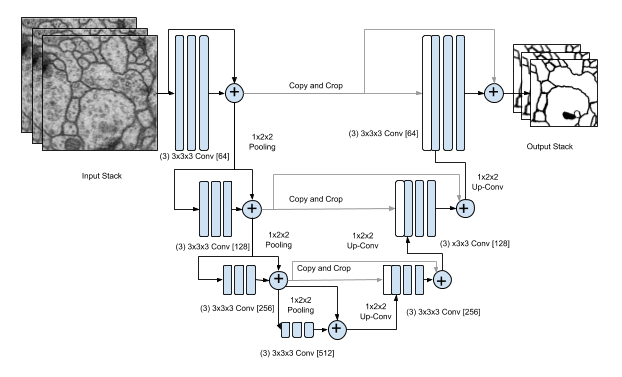
\includegraphics[width=\textwidth]{img/U-Net_3D.png}
	\caption{The UVR-Net architecture for 3D Segmentation}
	\label{fig:uvr-net}
	\end{figure}
\end{itemize}

\section{Dataset}

We will train and experiment on (4) 3D EM Datasets, taken from two different competitons: SNEMI3D and CREMI. We evaluate on 4 datasets instead of 1 to discuss the shortcomings of these models, and how training on different types of data affect performance.

The SNEMI3D Segmentation Challenge is a highly active 3D segmentation challenge (organized in advance of ISBI 2013), and provides a stack of EM images for training, along with ground truth segmentations of the EM images in 3 dimensions. The challenge website describes the training and testing data as \quotes{stacks of 100 sections from a serial section Scanning Electron Microscopy (ssSEM) data set of mouse cortex. The microcube measures 6 x 6 x 3 microns approx., with a resolution of 6x6x30 nm/pixel}\cite{Arganda-Carreras2013}. Like the ISBI 2012 dataset, the SNEMI3D dataset is anisotropic, and particularly dilated in the z-direction. Additionally, the data is from mouse cortex, rather than from \textit{Droposphilia}, and the geometry of the tissue is significantly different. 

The SNEMI3D dataset comes with a train and a test set, both of which consist of (100) 1024x1024 pixel images. The train set includes a set of labels, which represent a segmentation of the bodies in the stack. Since the test set does not include such a segmentation, we create a validation set of 25 images (25\%) which we will use to evaluate the performance of our models.

The Circuit Reconstruction from Electron Microscopy Images (CREMI) Challenge is a somewhat less-active challenge organized in advance of MICCAI 2016\cite{Funke.Jan2016}. The challenge provides three datasets for training, all of which are volumetric samples of \textit{Drosophila melanogaster}. The training and testing data are stacks of 125 sections from an ssSEM data set, with each slice having a resolution of 4x4x40nm/pixel. These datases are also anisotropic, being dilated in the z-direction. Furthermore, the types of neurons sampled are quite diverse between datasets: from visual inspection, some of the neurites in one of the datasets is much thinner than those in the others, suggesting that models might perform differently when trained/tested on these different datasets. Finally, these datasets are quite a bit noisier than ISBI or SNEMI3D: there are many more major misalignments, many patches of blur, and some slices are missing entirely. These datasets will provide a good measure of how robust our methods are to noise in volumetric data.

The three CREMI datasets (labeled CREMI A, CREMI B, and CREMI C) contain train and test sets, each of which consist of (125) 1250x1250 pixel images. The train set includes a set of labels, which represent a segmentation of the bodies in the stack. Like SNEMI3D, the test sets don't include segmentaitons, so we create validation sets from the training sets by witholding 25 slices (20\%) from each for evaluation of model performance.

\section{Training}

We train each model on each of the datasets, for a total of 8 training runs. Training was performed on a NVIDIA Titan X. We trained each net for 30000 iterations, sampling volumetric sections from each dataset that were 16 slices thick. For every model, we sought to minimize the cross entropy between the predicted affinities and the true afinnity labels, defining our loss function as:

$$\mathcal{L}(\bm{x}, \bm{y}) =-\log(\sigma(\bm{y}^{T}\bm{x}-(1-\bm{y}^{T})\bm{x}))$$
where $\sigma$ is the sigmoid function, $\bm{x}$ is the prediction, and $\bm{y}$ are the true affinites.

At each step, we executed one iteration of optimization using the Adam Optimizer, and ever 100 steps we made predictions on the validation set to see how well the model generalized.

\section{Results}


\begin{table}
	\centering
	\caption{Results of 3D Segmentation on various datasets}
	\subcaption*{SNEMI3D} 
	\begin{tabular}{lllll}
\toprule
{} & Pixel Error & Rand - Full & Rand - Merge & Rand - Split \\
\midrule
VD2D-3D &    0.102204 &    0.790909 &      0.95196 &     0.676465 \\
UVR-Net &   0.0863271 &    0.783288 &     0.993469 &     0.646511 \\
\bottomrule
\end{tabular}
 

	\subcaption*{CREMI A} 
	\begin{tabular}{lllll}
\toprule
{} &  Pixel Error &  Rand - Full &  Rand - Merge &  Rand - Split \\
\midrule
VD2D-3D &     0.098559 &     0.651105 &      0.981541 &      0.487117 \\
UVR-Net &     0.034879 &     0.576646 &      0.449545 &      0.803948 \\
\bottomrule
\end{tabular}
 

	\subcaption*{CREMI B} 
	\begin{tabular}{lllll}
\toprule
{} & Pixel Error & Rand - Full & Rand - Merge & Rand - Split \\
\midrule
VD2D-3D &    0.097363 &    0.845614 &     0.929446 &     0.775653 \\
UVR-Net &   0.0379261 &    0.846339 &     0.933393 &     0.774138 \\
\bottomrule
\end{tabular}
 

	\subcaption*{CREMI C} 
	\begin{tabular}{lllll}
\toprule
{} & Pixel Error & Rand - Full & Rand - Merge & Rand - Split \\
\midrule
VD2D-3D &     0.11817 &  0.00283098 &      0.91909 &   0.00141767 \\
UVR-Net &   0.0419219 &    0.748079 &     0.933252 &     0.624223 \\
\bottomrule
\end{tabular}
 
	
	\label{tab:3d_results}
\end{table}

\begin{figure}
\centering
\textbf{SNEMI3D} \\
\textbf{Rand Index}
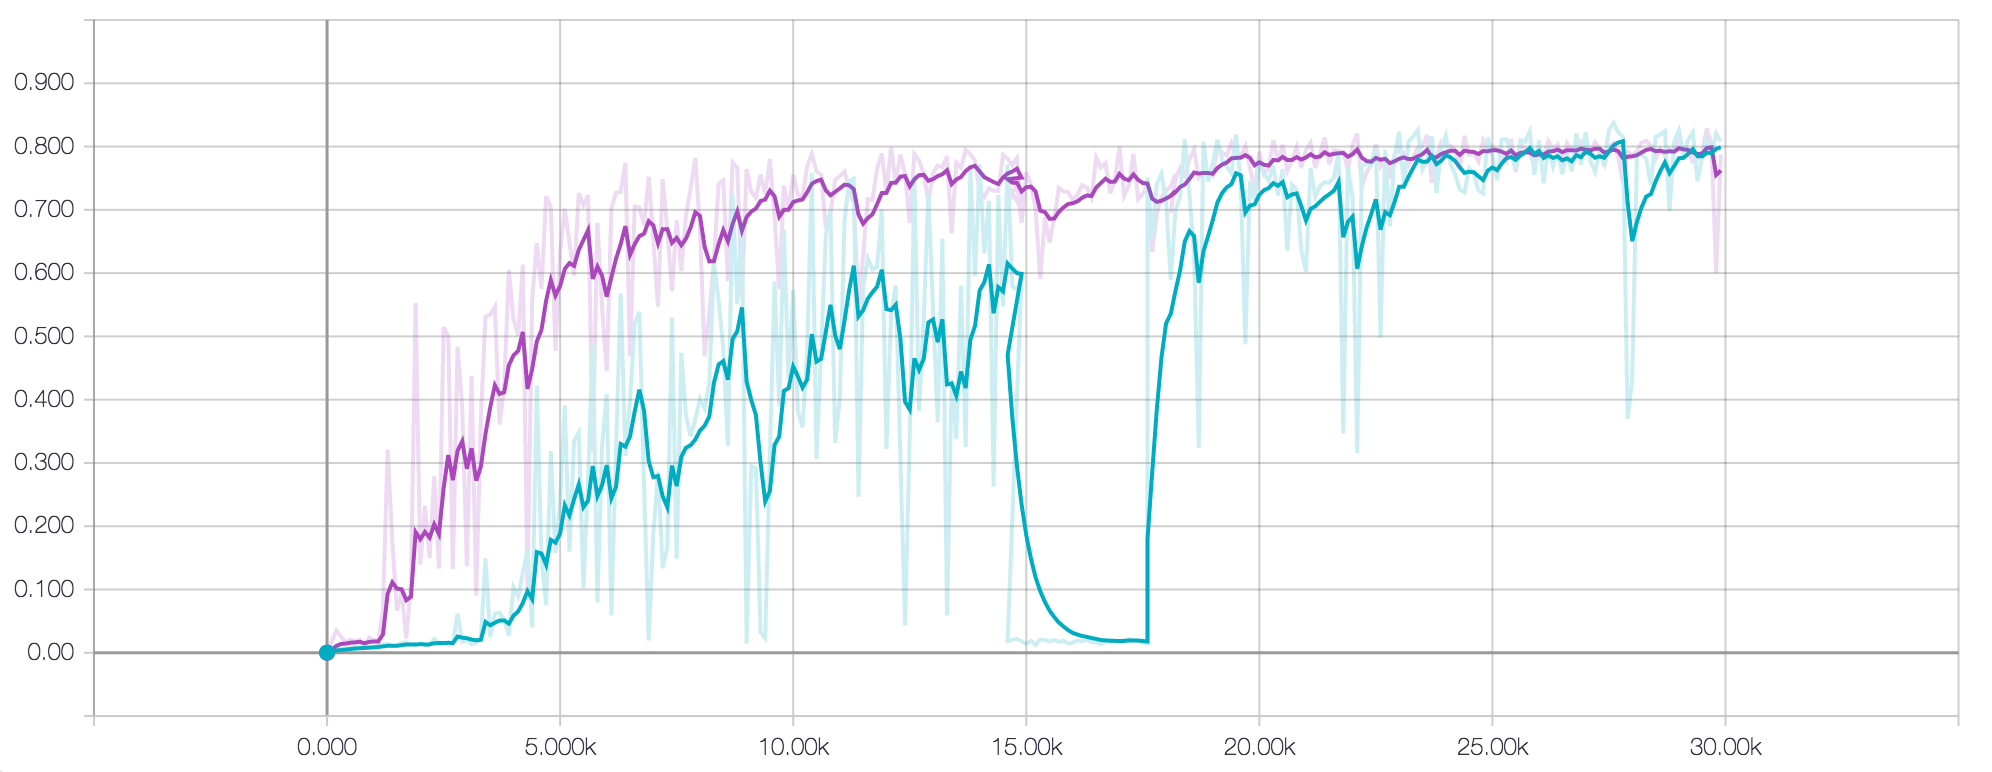
\includegraphics[width=\textwidth]{img/snemi_rand.png} \\
\textbf{Pixel Error}
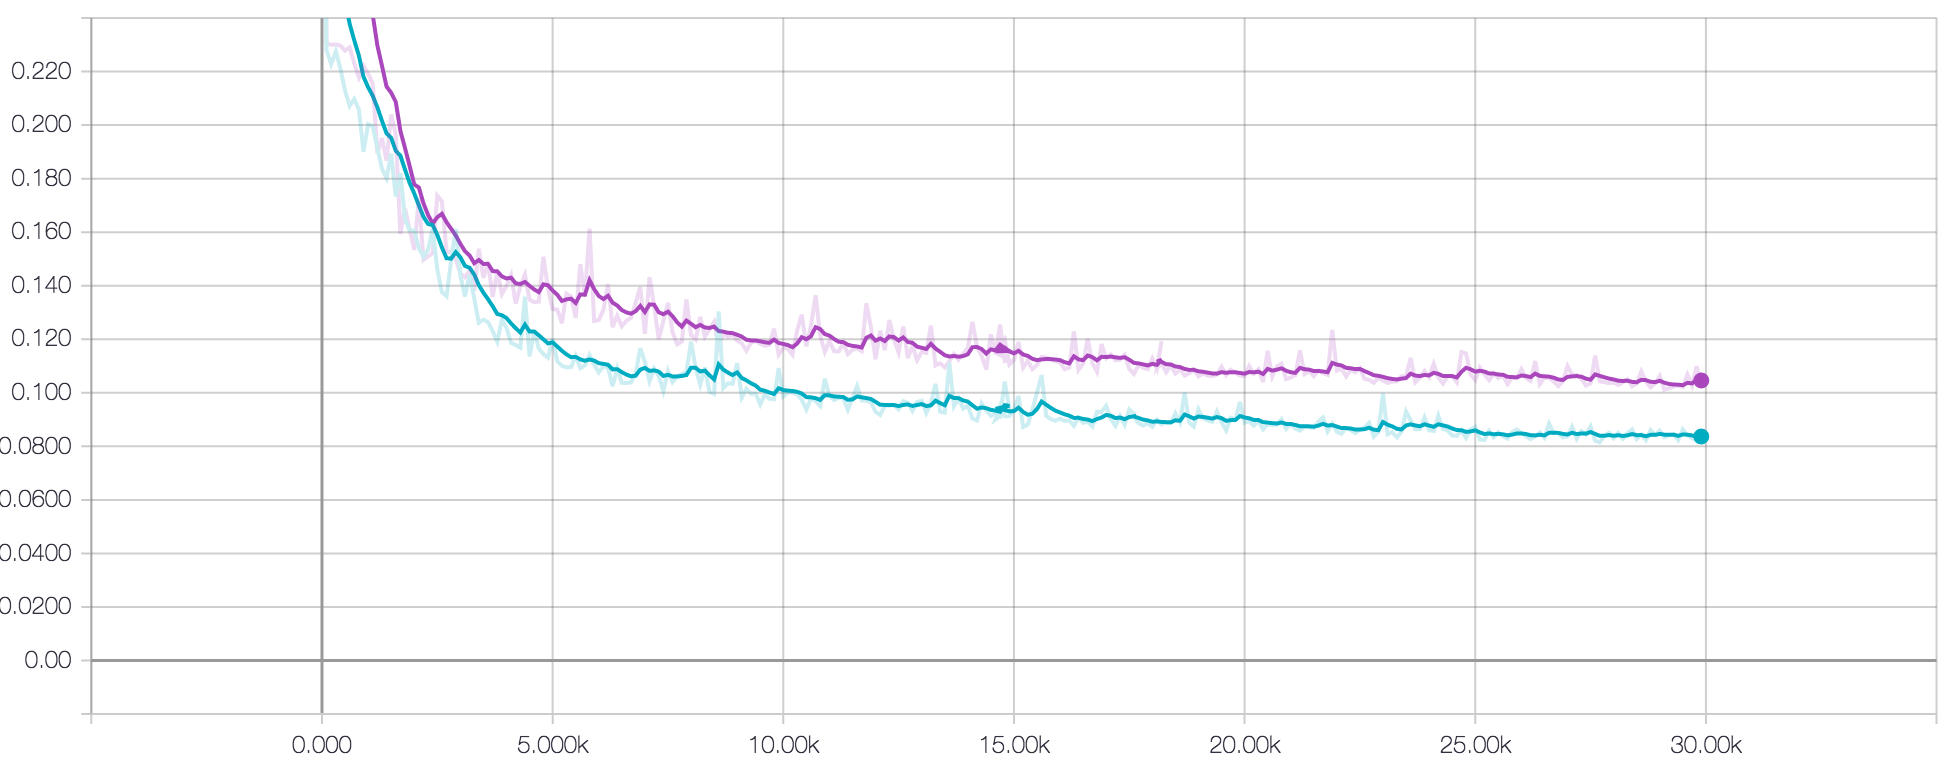
\includegraphics[width=\textwidth]{img/snemi_px_err.png}

\caption[Training curves for 3D segmentation for SNEMI3D]{Training curves, smoothed, for 3D segmentation. Top: The full Rand scores on the SNEMI3D validation set (from top: VD2D-3D, UVR-Net). Bottom: The pixel error on the SNEMI3D validation set (from top: VD2D-3D, UVR-Net). The sharp dip in the Rand Score for the UVR-Net was due to a small parameter change in validation procedure that was quickly reverted.}
\label{fig:snemi_training_curves}

\end{figure}

\begin{figure}
\centering
\textbf{CREMI A} \\
\textbf{Rand Index}
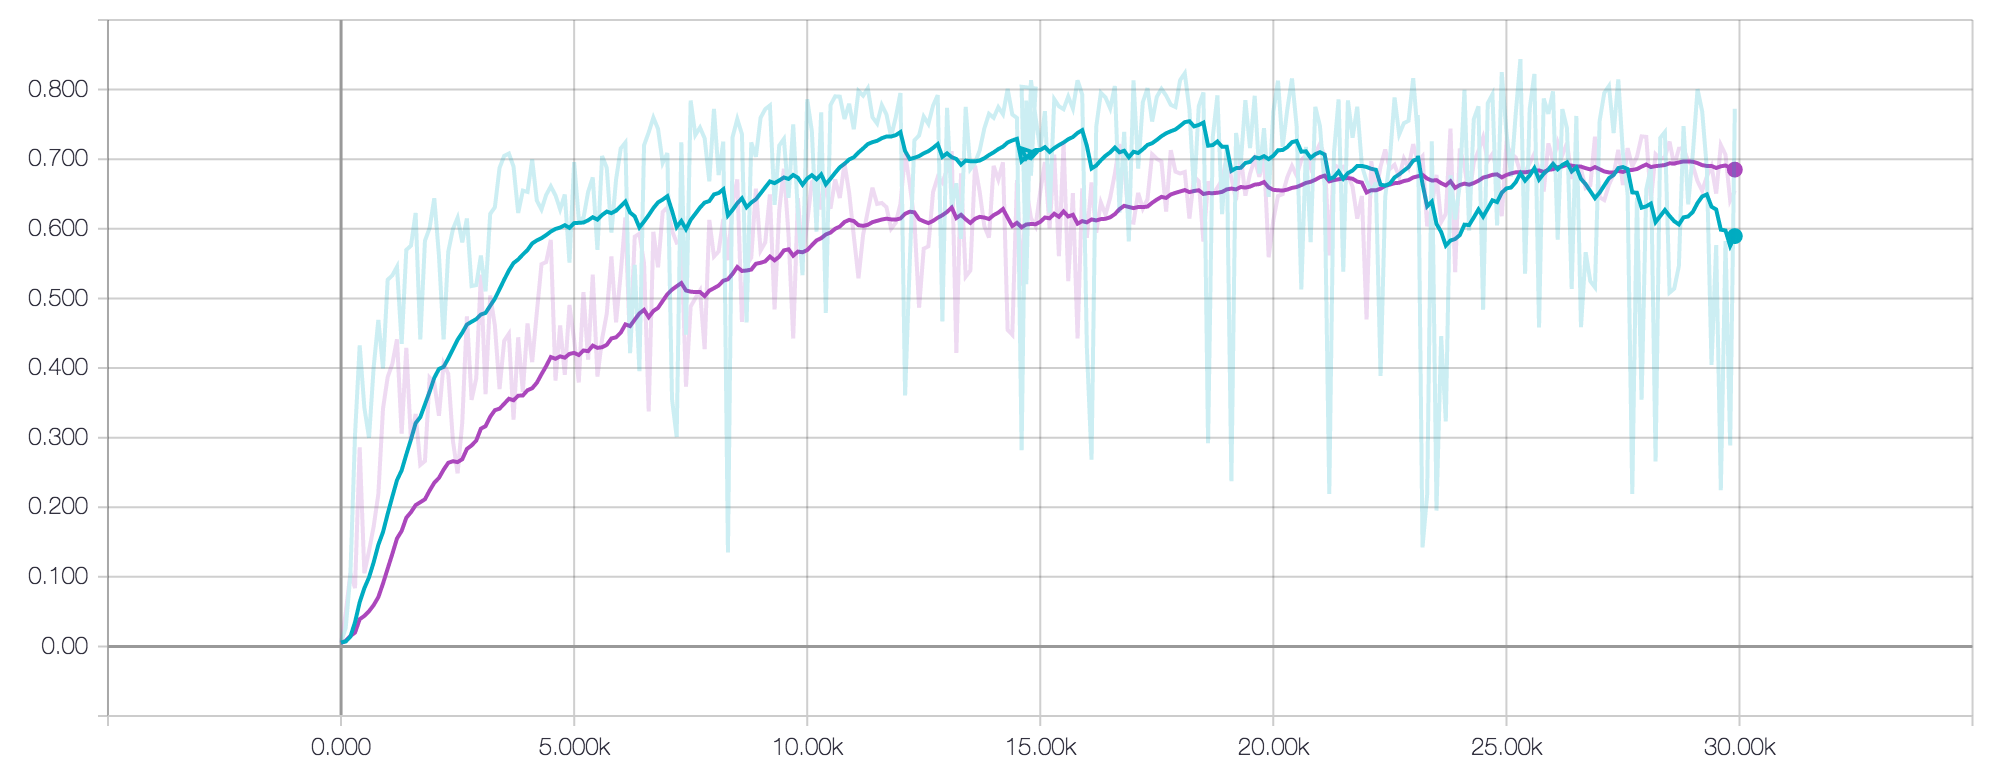
\includegraphics[width=\textwidth]{img/cremi_a_rand.png} \\
\textbf{Pixel Error}
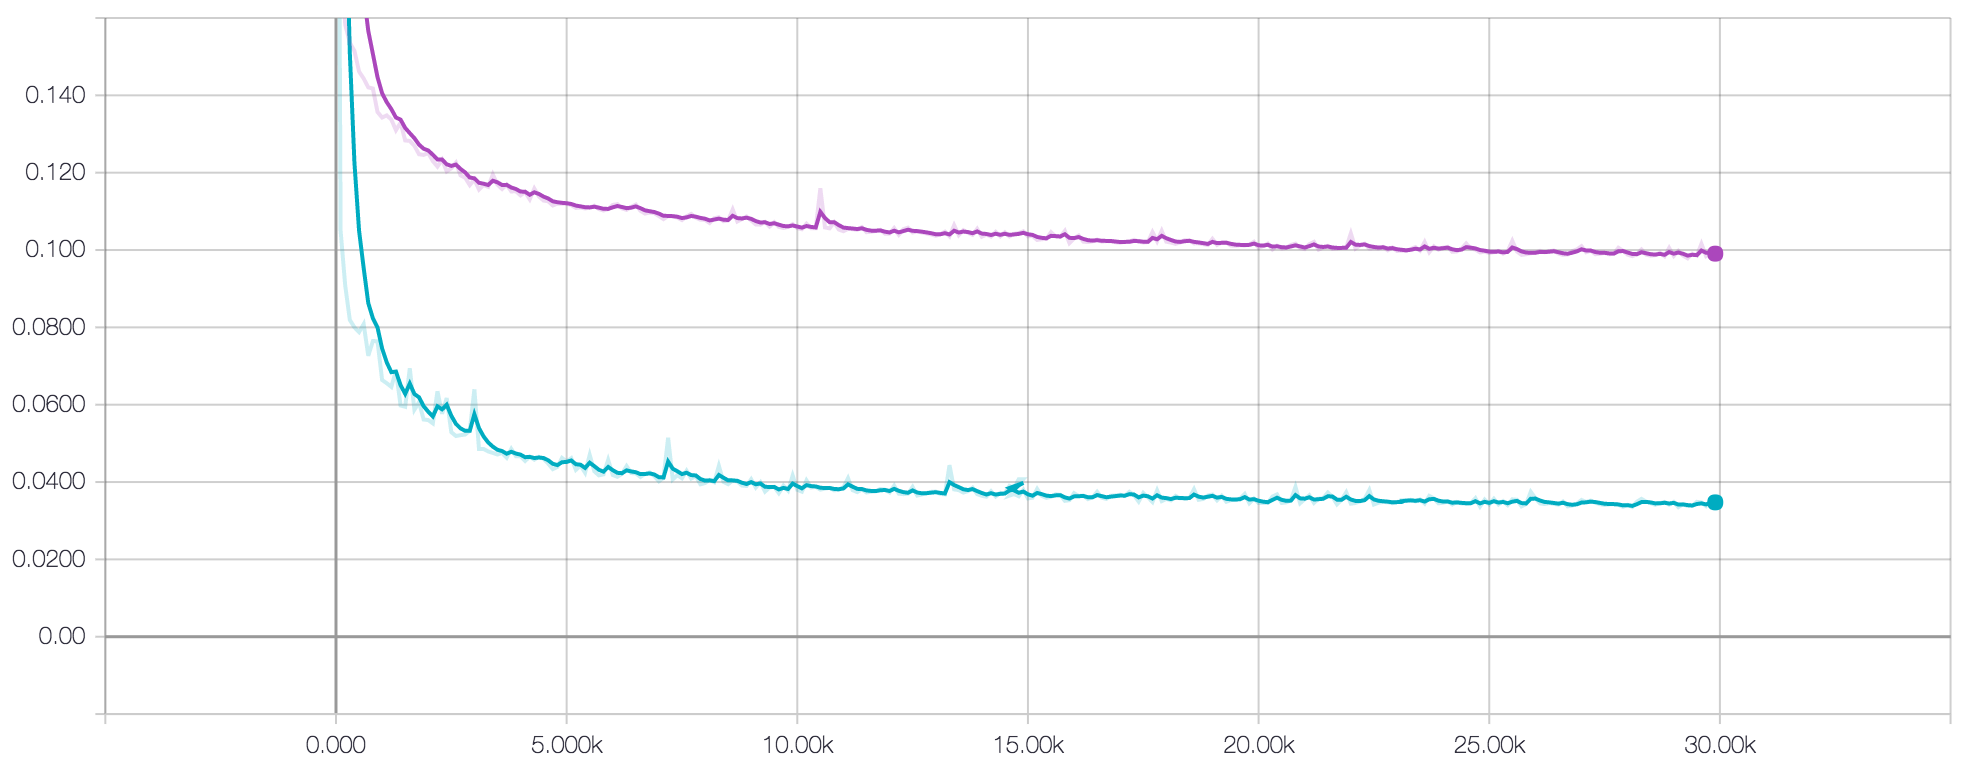
\includegraphics[width=\textwidth]{img/cremi_a_px_err.png}

\caption[Training curves for 3D segmentation for CREMI A]{Training curves, smoothed, for 3D segmentation. Top: The full Rand scores on the CREMI A validation set (from top: UVR-Net, VD2D-3D). Bottom: The pixel error on the CREMI A validation set (from top: VD2D-3D, UVR-Net).}
\label{fig:cremi_a_training_curves}

\end{figure}

\begin{figure}
\centering
\textbf{CREMI B} \\
\textbf{Rand Index}
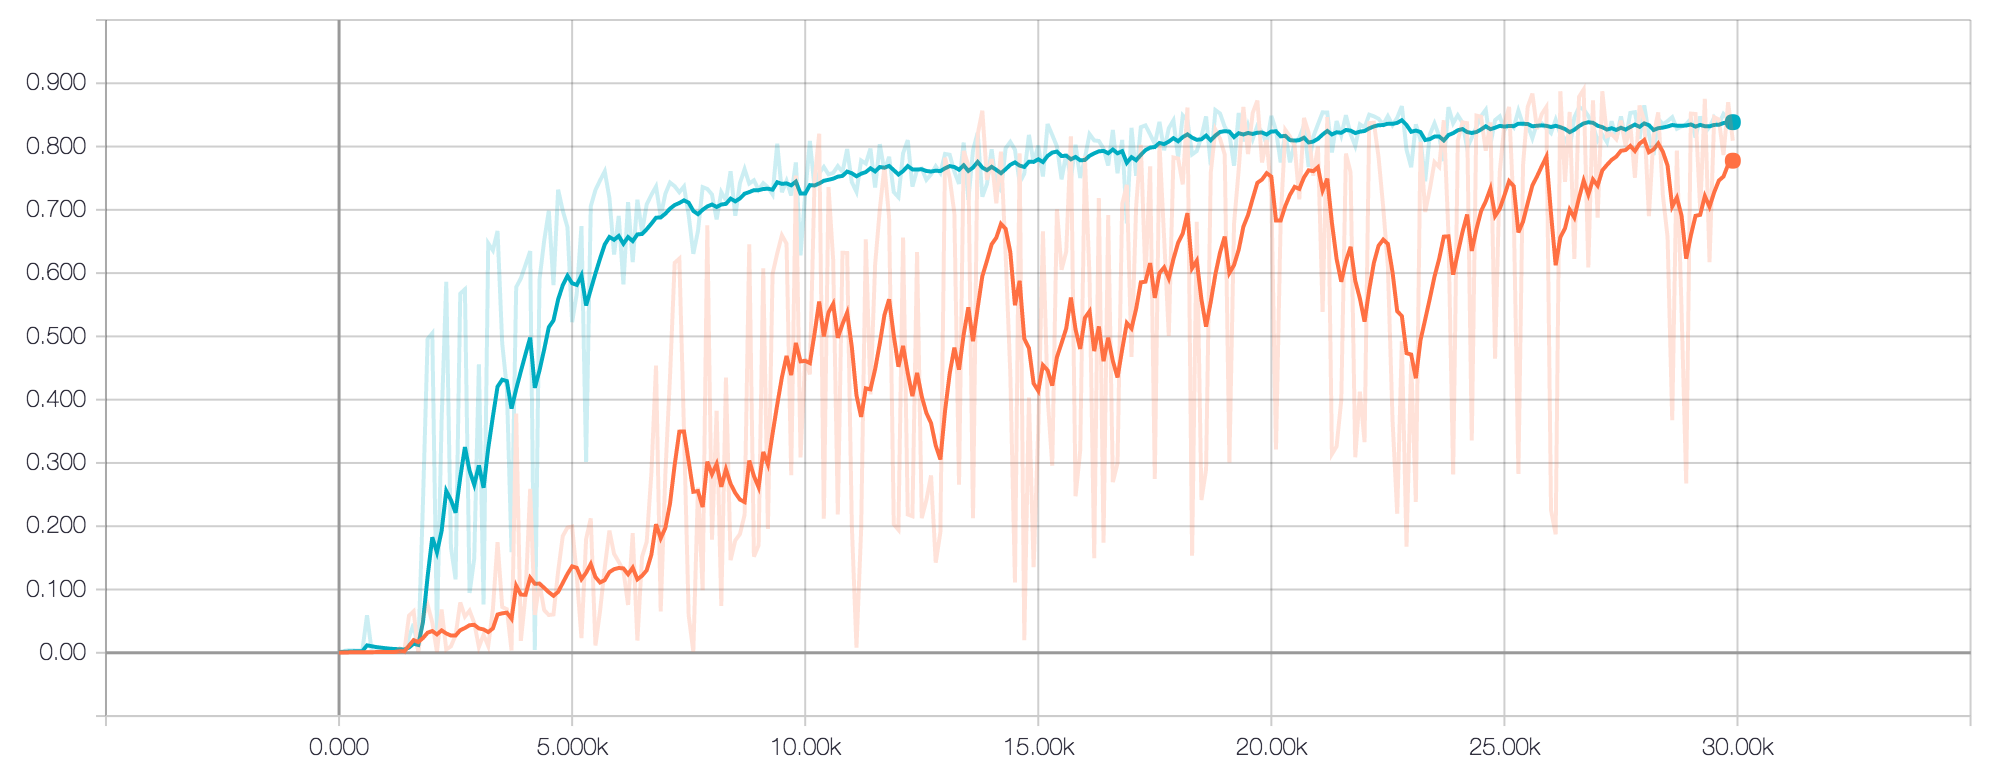
\includegraphics[width=\textwidth]{img/cremi_b_rand.png} \\
\textbf{Pixel Error}
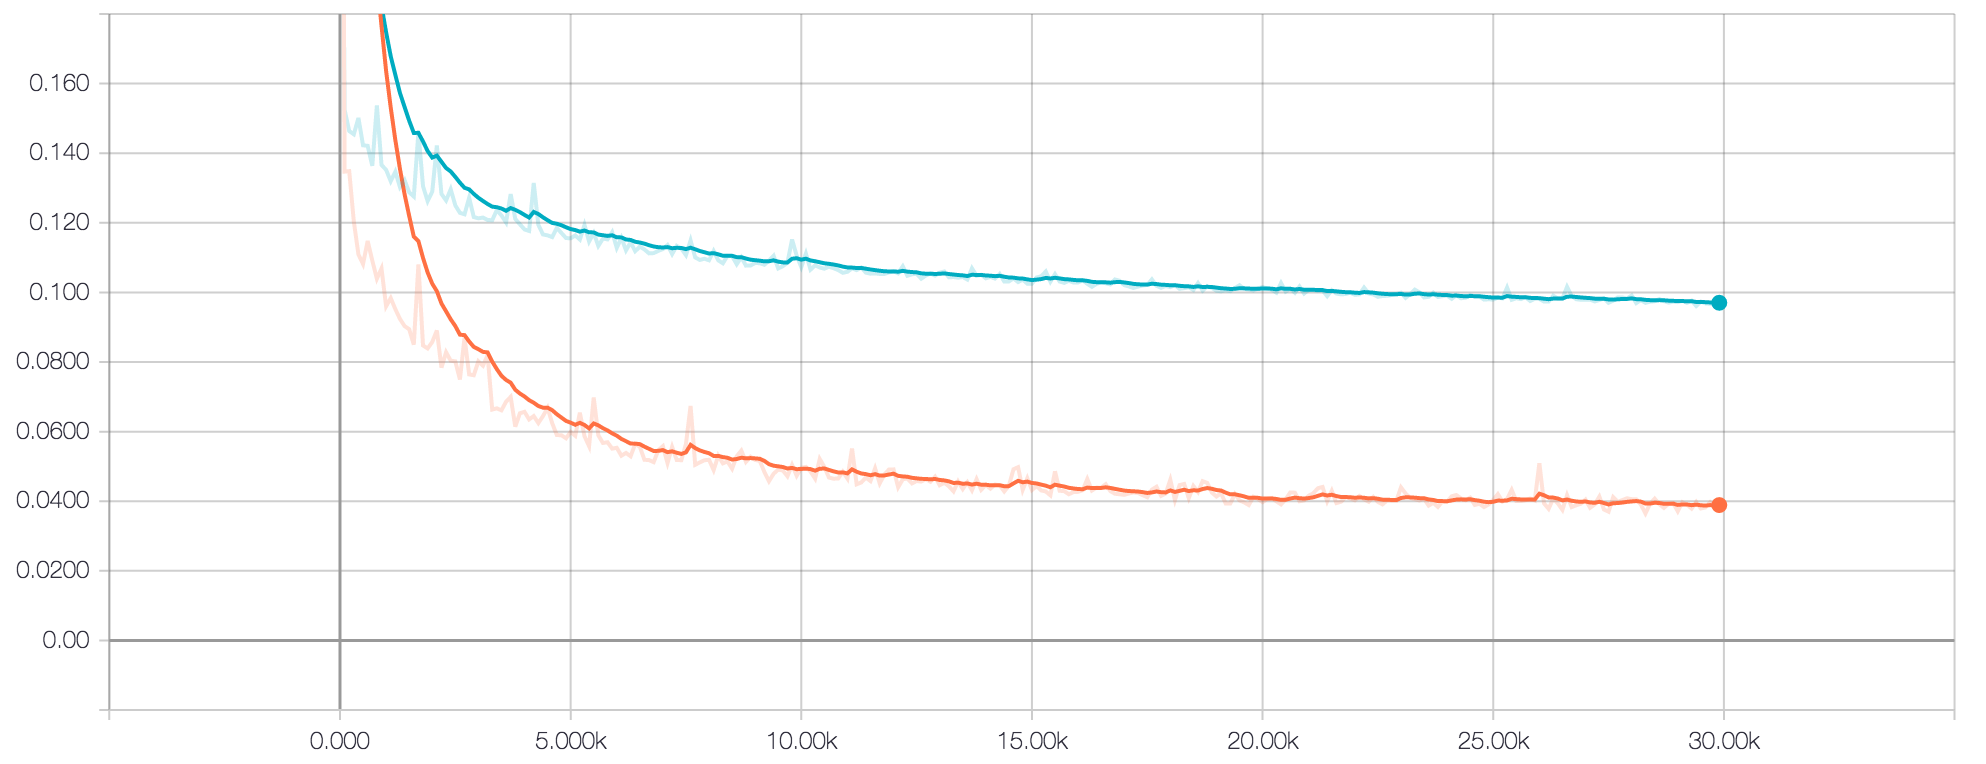
\includegraphics[width=\textwidth]{img/cremi_b_px_err.png}

\caption[Training curves for 3D segmentation for CREMI B]{Training curves, smoothed, for 3D segmentation. Top: The full Rand scores on the CREMI B validation set (from top: VD2D-3D, UVR-Net). Bottom: The pixel error on the CREMI B validation set (from top: VD2D-3D, UVR-Net).}
\label{fig:cremi_b_training_curves}

\end{figure}

\begin{figure}
\centering
\textbf{CREMI C} \\
\textbf{Rand Index}
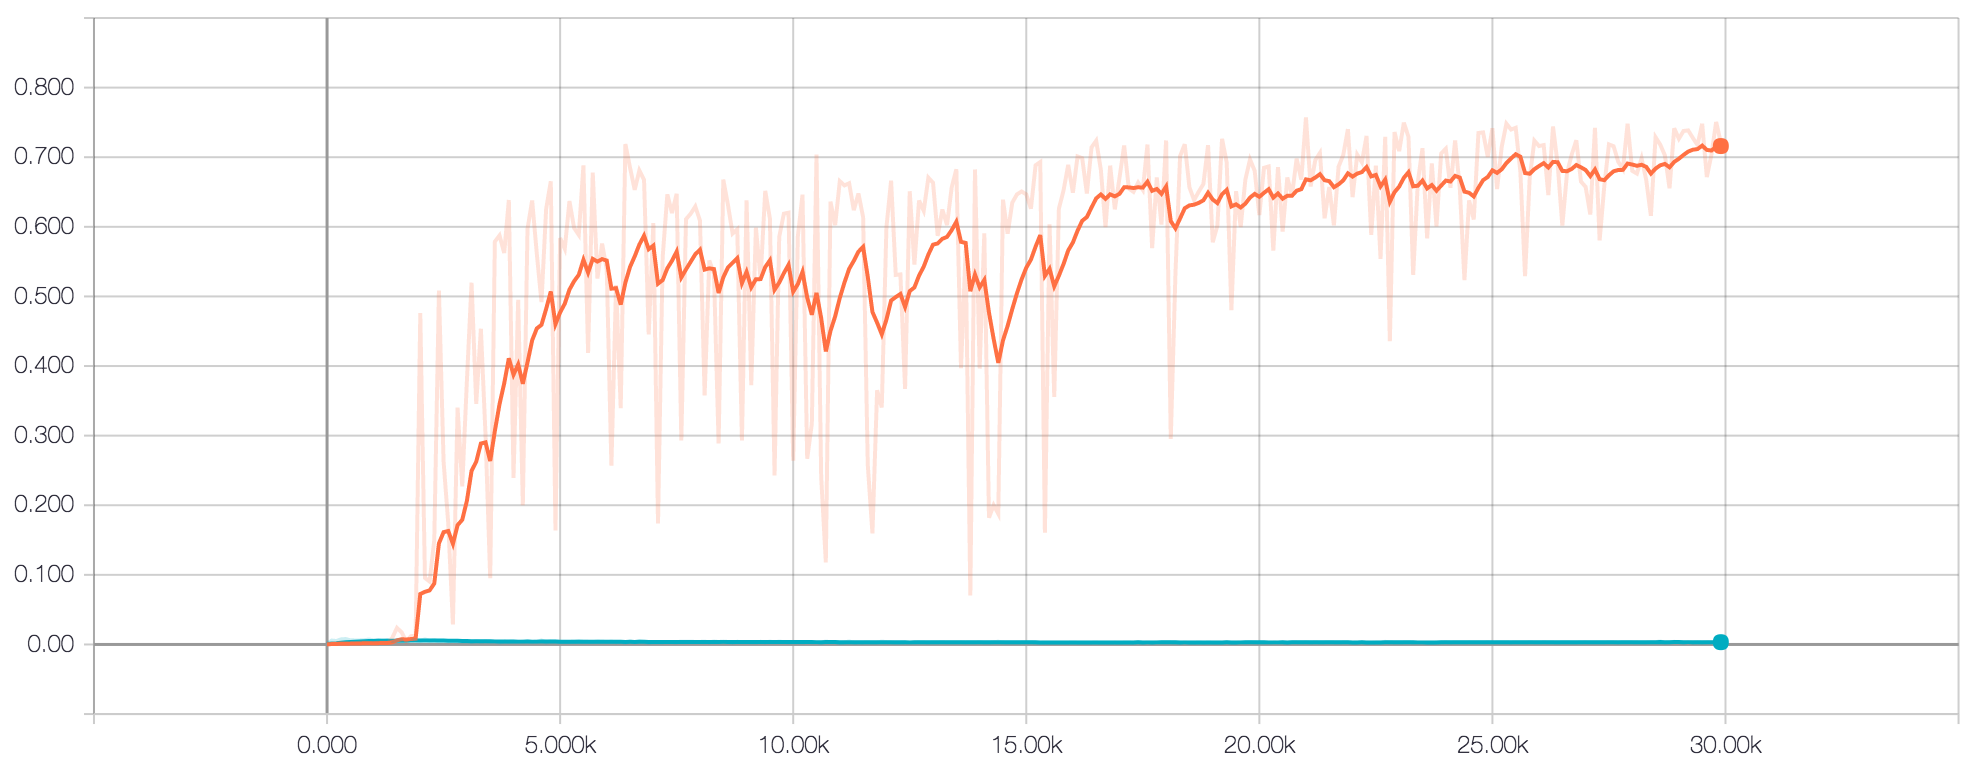
\includegraphics[width=\textwidth]{img/cremi_c_rand.png} \\
\textbf{Pixel Error}
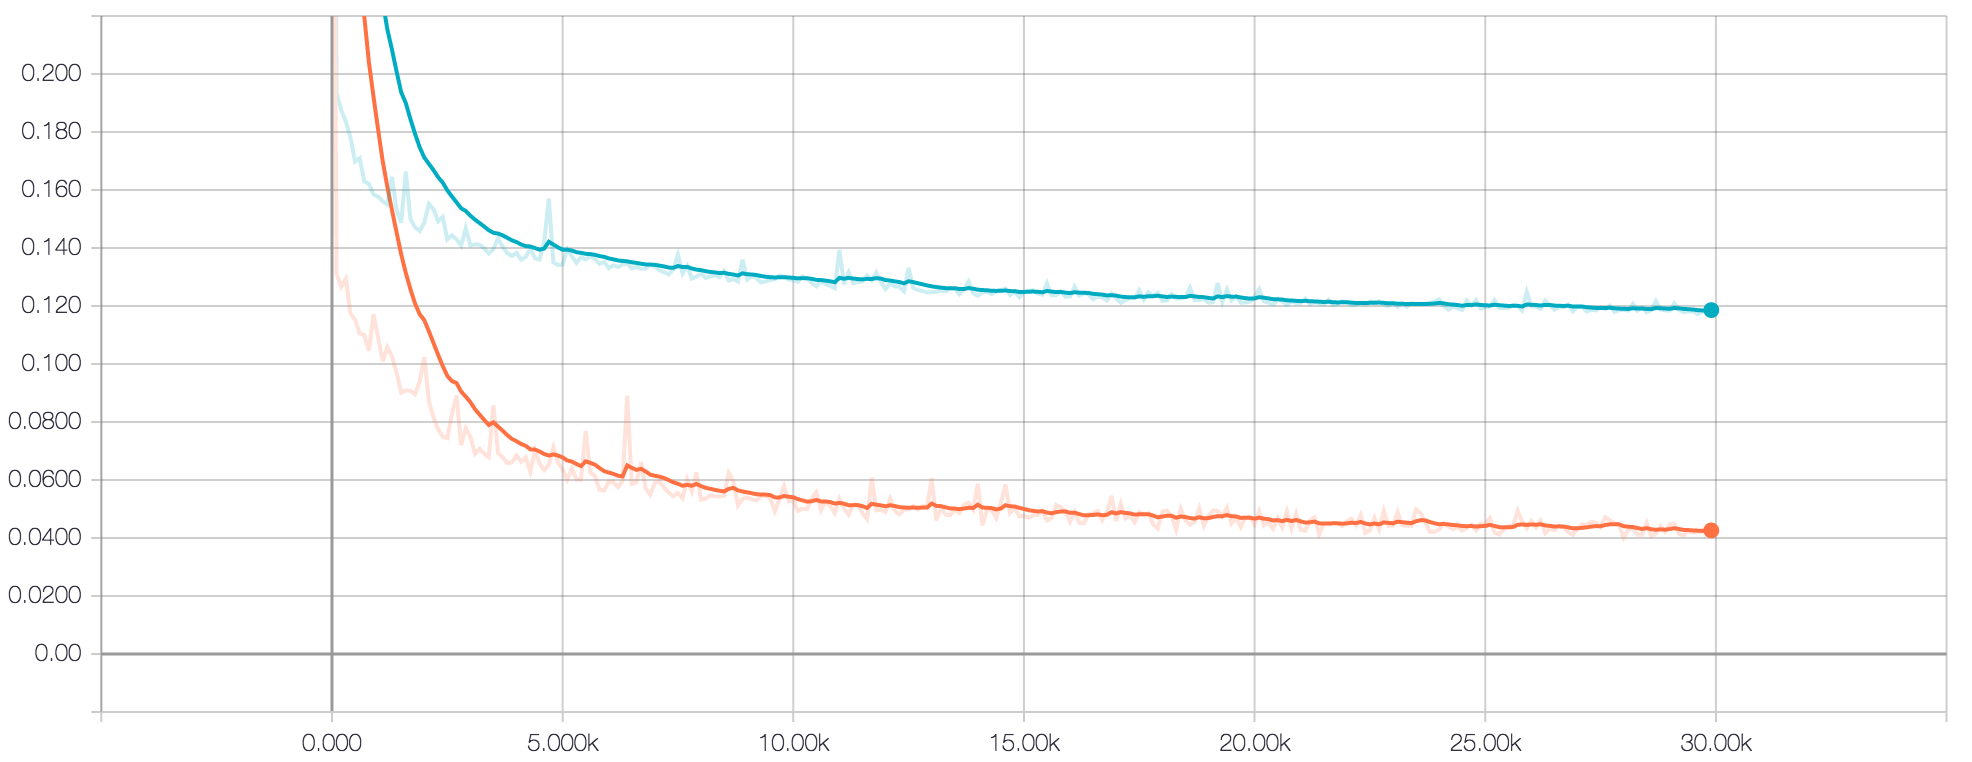
\includegraphics[width=\textwidth]{img/cremi_c_px_err.png}

\caption[Training curves for 3D segmentation for CREMI C]{Training curves, smoothed, for 3D segmentation. Top: The full Rand scores on the CREMI C validation set (from top: UVR-Net, VD2D-3D (barely pictured)). Bottom: The pixel error on the CREMI C validation set (from top: VD2D-3D, UVR-Net). The absurdly low Rand score for the VD2D-3D model might be a bit misleading; it is possible that there was a training fluke for this iteration.}
\label{fig:cremi_c_training_curves}

\end{figure}


After training, we run prediction on the validation sets for each dataset (since we don't have labels for the test set) to determine their performance. Results are numerically summarized in Table \ref{tab:3d_results}. The training graphs documenting Rand Score and Pixel Error for models training on SNEMI3D, CREMI A, CREMI B, and CREMI C can be found in Figures \ref{fig:snemi_training_curves}, \ref{fig:cremi_a_training_curves}, \ref{fig:cremi_b_training_curves}, and \ref{fig:cremi_c_training_curves}, respectively. 

We can draw several conclusions about the qualities that these models have when trained on these datasets. First, it is patently obvious that there is large variation in the training process. Sometimes, the models would train quite quickly; sometimes, they wouldn't train appropriately (in the case of VD2D-3D on CREMI C). If we were to repeat this study, we would likely train each model on each dataset multiple times with the same parameters, and take the best performing model from each set of runs. 

Second, in every setting the UVR-Net outperforms the VD2D-3D net in Pixel Error; UVR-Net consistently has substantially lower pixel error than VD2D-3D, by about the same margin in every trial. This suggests that the residual layers and skip connections built into the architecture are doing their jobs, and are reconstructing images that look a lot like the input (an affinity map should look quite like the boundaries of the input). 

Thrid, the quality of the data significantly affects the performance of these models. While some of the differences in scores can be attributed to variance in the training of the model, during the experimentation process (before results generation) it became clear that models would perform differently on different datasets. From this, we can draw the conclusion that certain datasets are "harder" than others to learn segmentatons from. What makes one dataset "harder" than another? 

In the SNEMI3D dataset, for instance, many of the objects are significantly thinner and extend longer distances across the EM slices than in the other datasets. Data quality can make a huge difference as well. The three different CREMI datasets, although taken from the same biological sample and imaged with the same process, have different properties in terms of stack quality. Visually looking at each layer of the CREMI stacks, the quality of the images varies greatly. Some of the CREMI datasets have significantly more blurred slices than others; the same goes for blemishes and cracks. CREMI C is missing a slice entirely. Individual slice artifacts may have a small impact on final metrics, but it is likely that only dataset errors affecting many slices across a dataset will have significant impact on the Rand Score of predictions. The most obvious culprit between the CREMI datasets is alignment. All three datasets are poorly aligned across the entire stack, but in terms of alignment CREMI A is worse than CREMI B and CREMI C. The Rand scores on CREMI A were also lower across all models than the other CREMI datasets. While this is not concrete evidence that the models are quite susceptible to error on poorly aligned datasets, the correlation certainly suggests that improving alignment procedures for EM datasets, or even building explicit alignment layers into models might produce better results across diverse datasets.

\chapter{Alignment}

\section{Task Definition}


One major hurdle in inferring neural structure from EM images is that the image acquisition process is inherently noisy. While the EM imaging technologies used for the creation of neuron images (typically TEM) are quite stable, there is often variance in sample preparation techniques, resulting in all sorts of distortions and errors at imaging time. One particular type of error, image misalignment, occurs during the slicing of sample tissue, when some physical factor causes a resulting slice to be warped or translated in such a way that the resulting stack of images is misaligned. Intuitively, this means that every point in one EM slice data does not necessarily map to the point directly below it the neighboring slice. An example of slice misalignment can be visualized in Figure \ref{fig:misalignment_example}.

\begin{figure}[h]
    \centering
	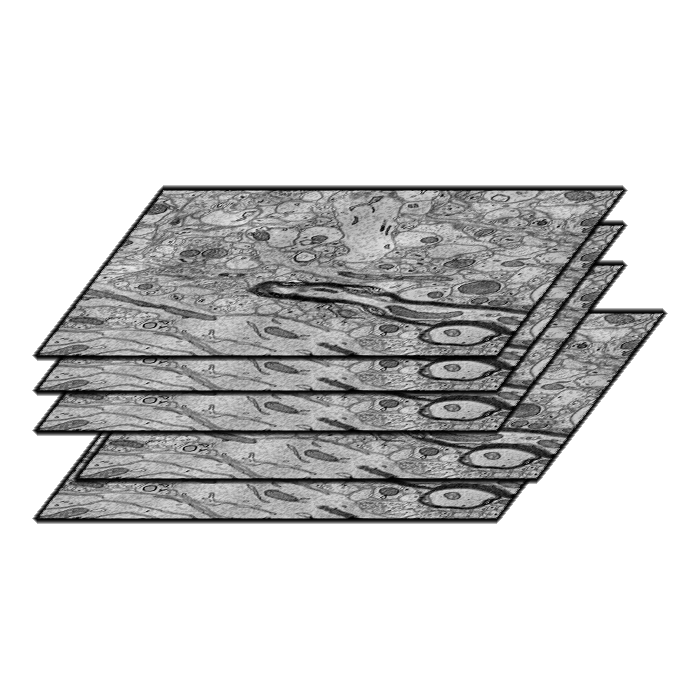
\includegraphics[width=0.33\textwidth]{img/misalignment_example}
	\hspace{1cm}
	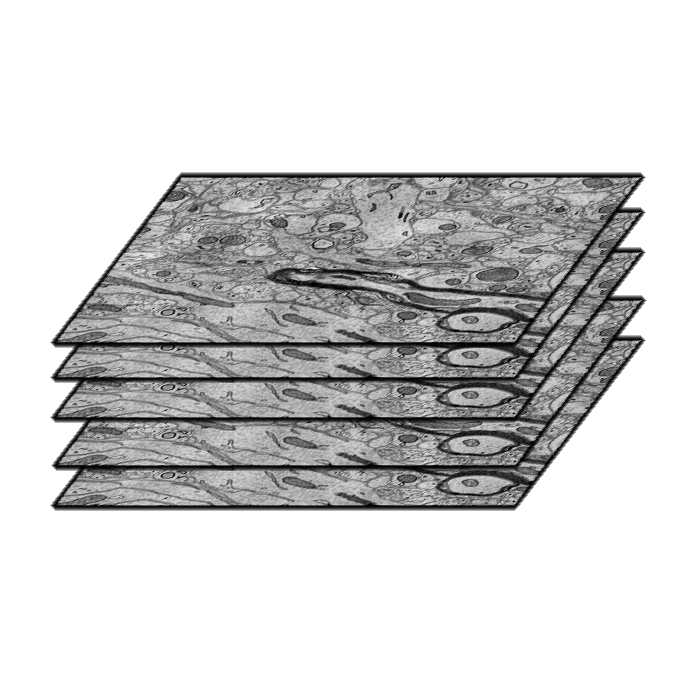
\includegraphics[width=0.33\textwidth]{img/alignment_example}
    \caption[An example of a 3D stack of EM images that contains a misalignment]{An example of a 3D stack of EM images that contains a misalignment. Left: The provided alignment of a stack. This represents a misalignment where the fourth image in a stack of images actually represents a slice slightly translated in position. Right: The correct alignment of the stack, where all the pixels in the fourth position have been translated enough such that the structures depicted in the input data line up in the z-direction.}
    \label{fig:misalignment_example}
\end{figure}

The problem of misalignment within a set of EM images particularly induces problems in the task of 3D Segmentation. While most techniques are rather invariant to small misalignments (particularly CNNs, which can be trained to be invariant to warping of many kinds), large misaligments can often induce false splitting in segmentations. Very deep CNNs trained with a really diverse set of data would likely be able to compensate for these sorts of misalignments, but it would be more prudent to develop a more efficient strategy for automatically healing misalignments in the data. 

\section{Evaluation Metrics}

\section{Models}

\section{Dataset}

\section{Training}

\section{Results}
\chapter{Conclusion}


\appendix % all chapters following will be labeled as appendices
\chapter{Metric Definitions}

\section{Pixel Error}
Given two images, pixel error is defined as the mean of the absolute numerical distance between corresponding pixels in both images. Formally, we define:

$$P(X, Y) = \frac{\sum_{\bm{i} \in S}{|X_{\bm{i}} - Y_{\bm{i}}|}}{|S|}$$
for tensors $X$ and $Y$ over all indexes $\bm{i}$ in the index space $S$ for tensors $X$ and $Y$.

\section{Rand Score}

The version of the Rand Score used in this thesis is the Rand F Score. The Rand F Score essentially counts all the non-distinct pairs in an image that are correctly labeled as belonging to the same or different grouping with respect to a reference image. Formally, we define $S_1, S_2, ... S_n \subseteq S$ to be the set of all groupings $S_i$ in an input volume (i.e. distinct labels in a segmentation)m and $T_1, T_2, ... T_n \subseteq T$ to be the set of all groupings $T_i$ in a ground-truth volume. Let:

$$ t_i = |T_i| $$
$$ s_i = |S_i| $$
$$ c_{i,j} = |S_i \cap T_j| $$

Then, the Rand F Score can be defined as:

$$R_{\mathsf{Full}}(S,T) = \frac{\sum_{i,j}{c_{i,j}}}{\alpha \sum_{i}{s_i^2} + (1 - \alpha)\sum_j{t_i^2}}$$ 

$$R_{\mathsf{Merge}}(S,T) = \frac{\sum_{i,j}{c_{i,j}}}{\sum_{i}{s_i^2}}$$  

$$R_{\mathsf{Split}}(S,T) = \frac{\sum_{i,j}{c_{i,j}}}{\sum_{j}{t_j^2}}$$  


where $N$ is the number of voxels in a volume. See \url{https://github.com/seung-lab/segascorus/blob/master/segerror-manual.pdf} for more details of the Rand F Score.

\section{Cross Correlation}

Given two images, cross-correlation is defined as the mean of the prodiuct of corresponding pixels in both images. Formally, we define:

$$C(X, Y) = \frac{\sum_{\bm{i} \in S}{|X_{\bm{i}} \times Y_{\bm{i}}|}}{|S|}$$
for tensors $X$ and $Y$ over all indexes $\bm{i}$ in the index space $S$ for tensors $X$ and $Y$.

\subsection{Smoothed Version}

Because standard Cross Correlation is not particularly continuous (i.e. two images will typically be highly correlated if they match exactly, and loosely correlated if they are translated or rotated), we define a somewhat more smoothed version that attempts to make the function more continuous. We define the function:

$$C_s(X, Y) = \frac{\sum_{\bm{i} \in S}{|X_{\bm{i}} \times (G_{\theta}(Y))_{\bm{i}}|}}{|S|}$$
for tensors $X$ and $Y$ over all indexes $\bm{i}$ in the index space $S$ for tensors $X$ and $Y$. The function $G_{\theta}(\cdot)$ is a smoothing function, which applies a Gaussian filter to its arguments based on parameters $\theta$. The amount of smoothing that occurs determines how dontinuous the smoothed cross-correlation function is. Because the continuity of this function can be controlled, it makes for a more-useful loss function than standard Cross Correlation.


% Make the bibliography single spaced
\singlespacing
\bibliographystyle{plain}

% add the Bibliography to the Table of Contents
\cleardoublepage
\ifdefined\phantomsection
  \phantomsection  % makes hyperref recognize this section properly for pdf link
\else
\fi
\addcontentsline{toc}{chapter}{Bibliography}

% include your .bib file
\bibliography{SeungLab}

\end{document}